\chapter{モジュール設計}
\section{前提}
我々は\texttt{Ruby on rails}を用いて開発を行う.この言語の慣習にのっとり,これ以降,
\begin{itemize}
    \item index
    \item new
    \item show
    \item edit
    \item create
    \item destroy
    \item home
\end{itemize}
の7つは「アクション」と呼び,これ以外の関数をすべて「メソッド」と呼ぶ.\par
アクションはコントローラが異なれば同名のものを使用するため,モジュールIDを「Controller名.アクション名」
とする.また,1アクション1機能を持つ.

\section{モジュール詳細}
以下に,各モジュールについて「定義書」「フロー図」の順で示す.


%index
\begin{figure}
    \centering
    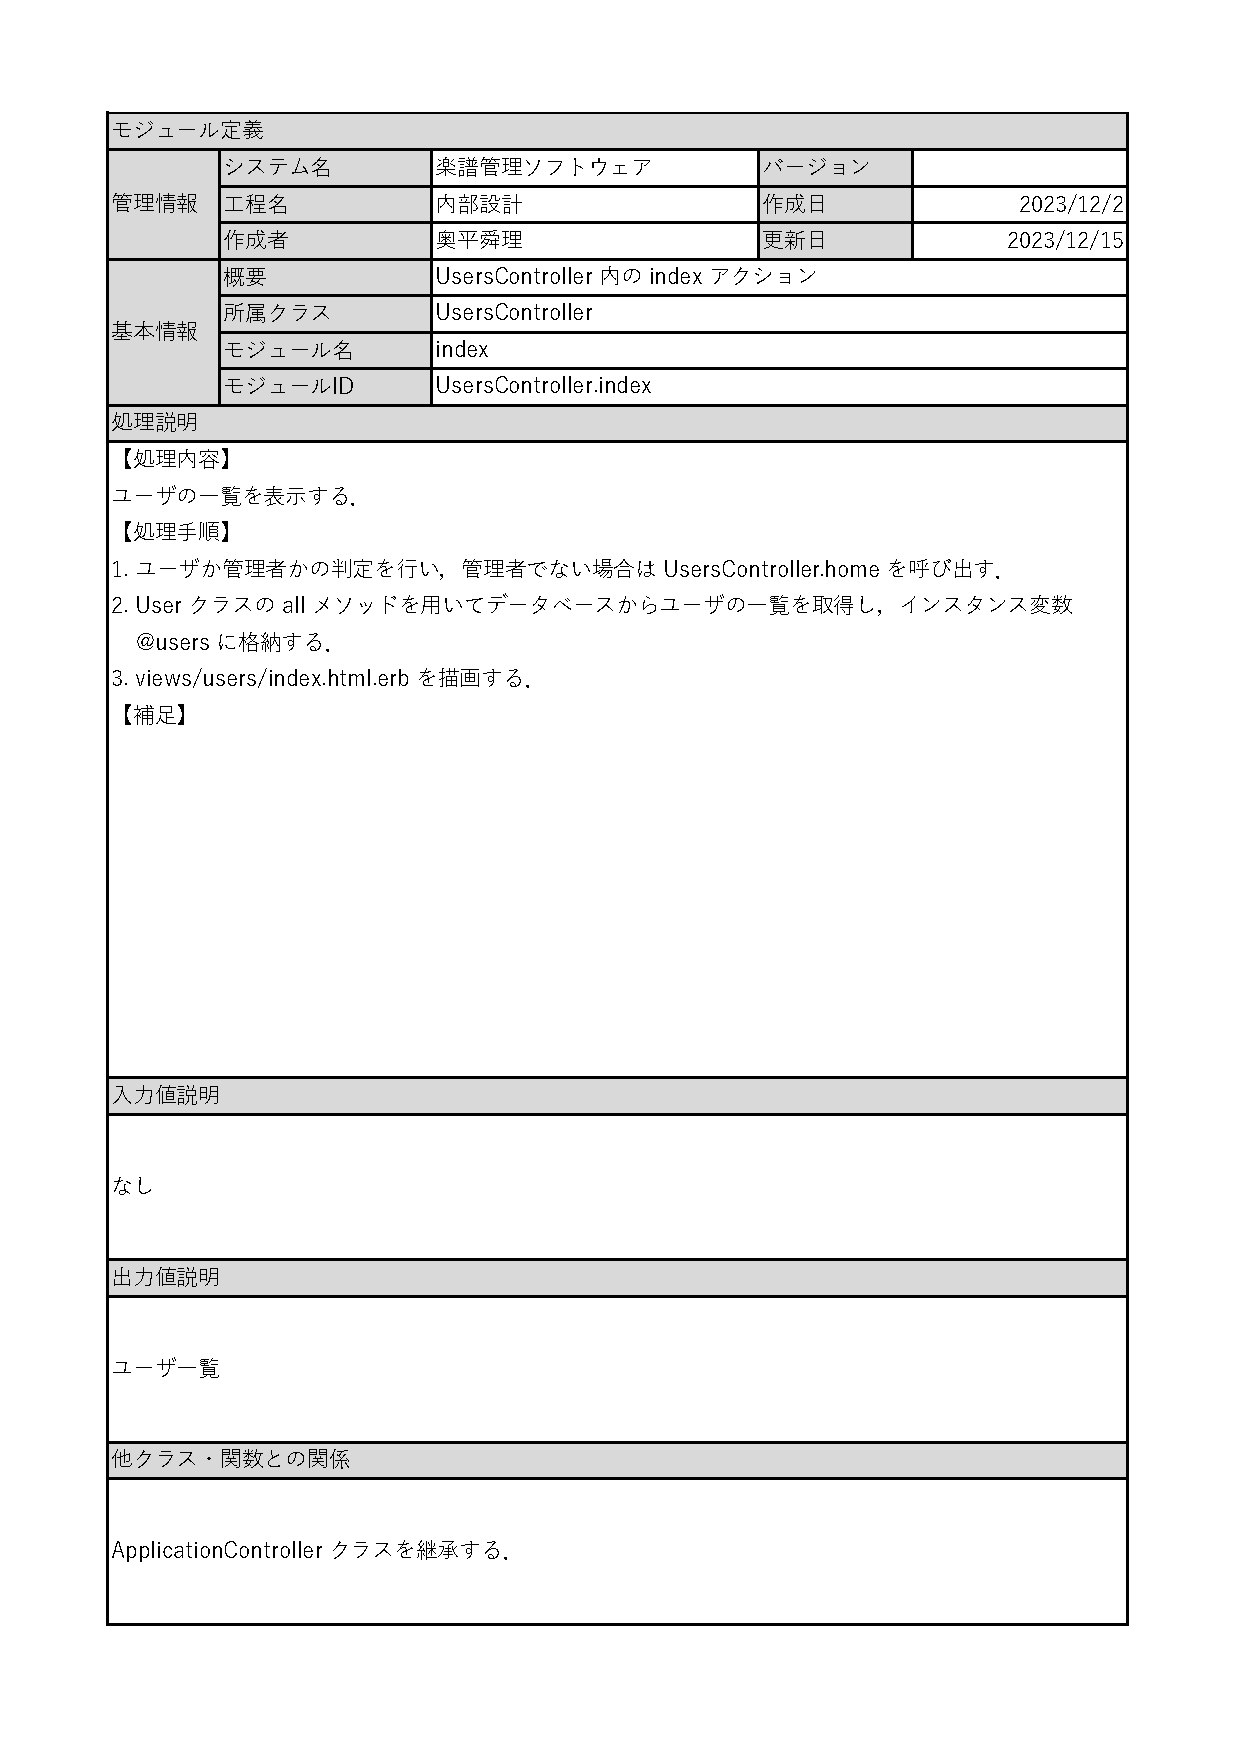
\includegraphics[scale=0.7]{img/Users/xlsx/UsersController_index.pdf}
    \vspace{-1cm}
    \caption{UsersController.index定義書}
\end{figure}
\begin{figure}
    \centering
    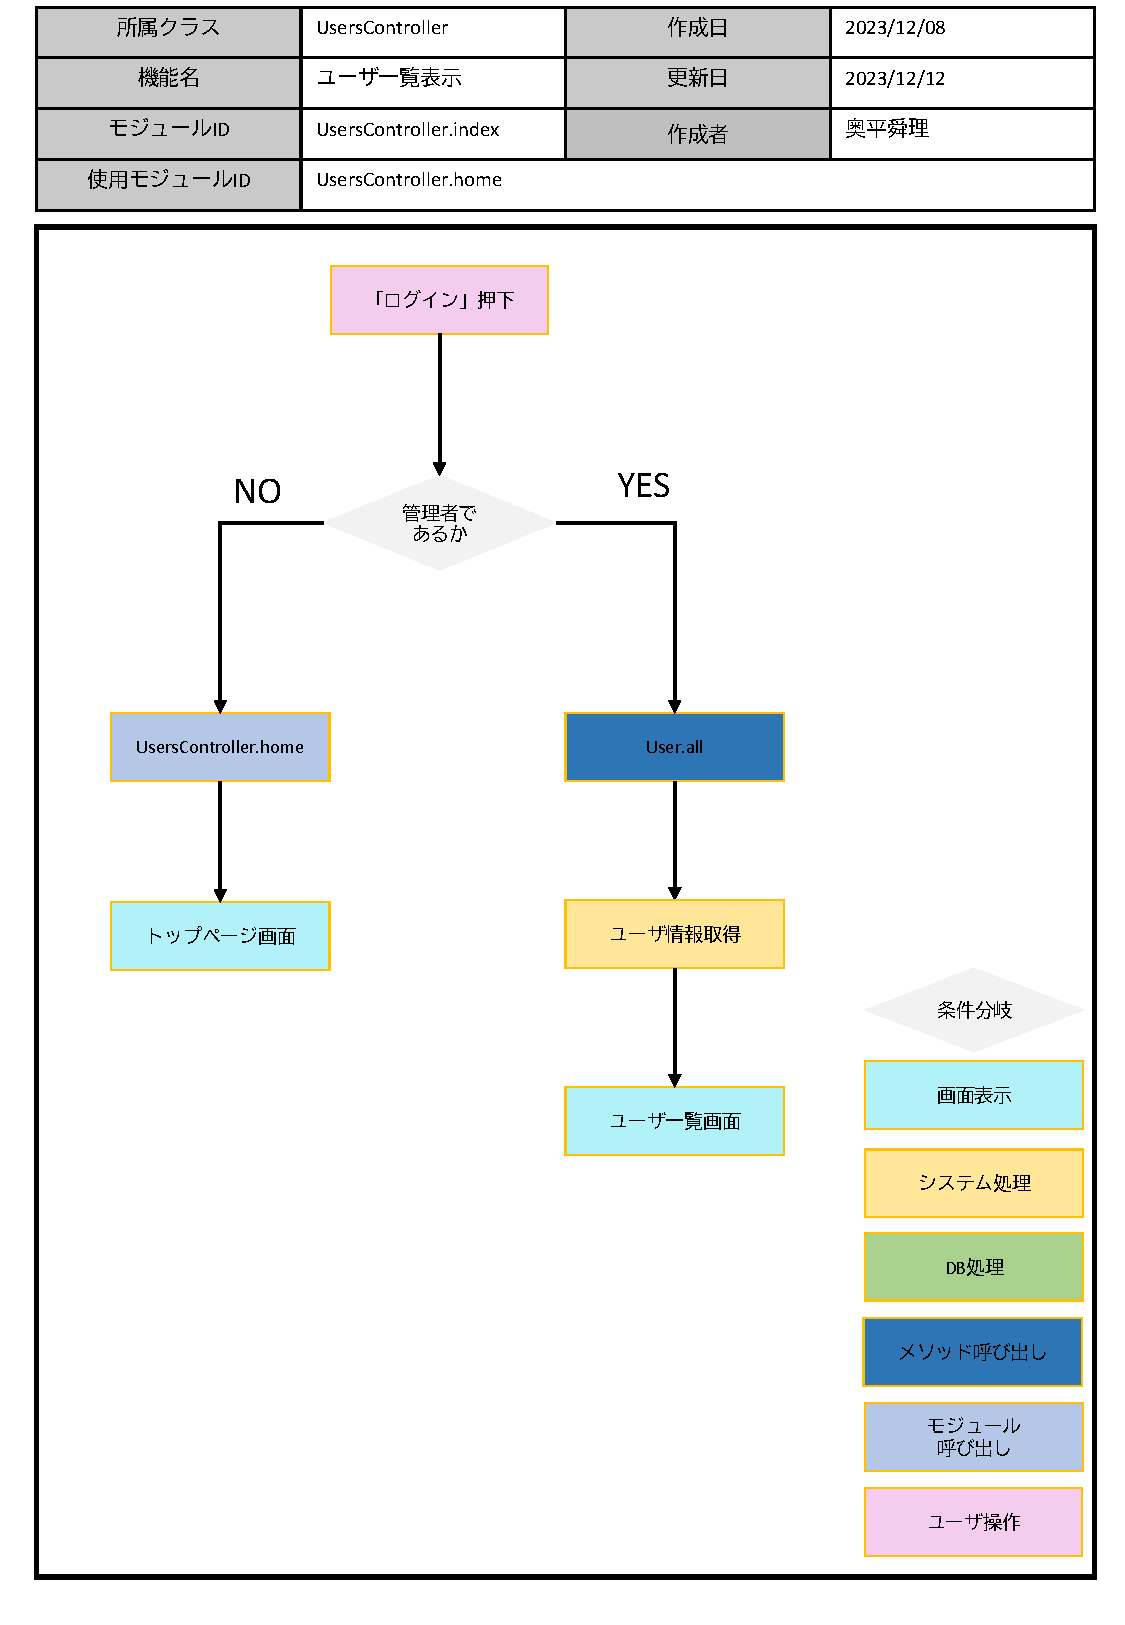
\includegraphics[scale=0.7]{img/Users/pptx/UsersController_index.pdf}
    \caption{UsersController.indexフロー図}
\end{figure}
\begin{figure}
    \centering
    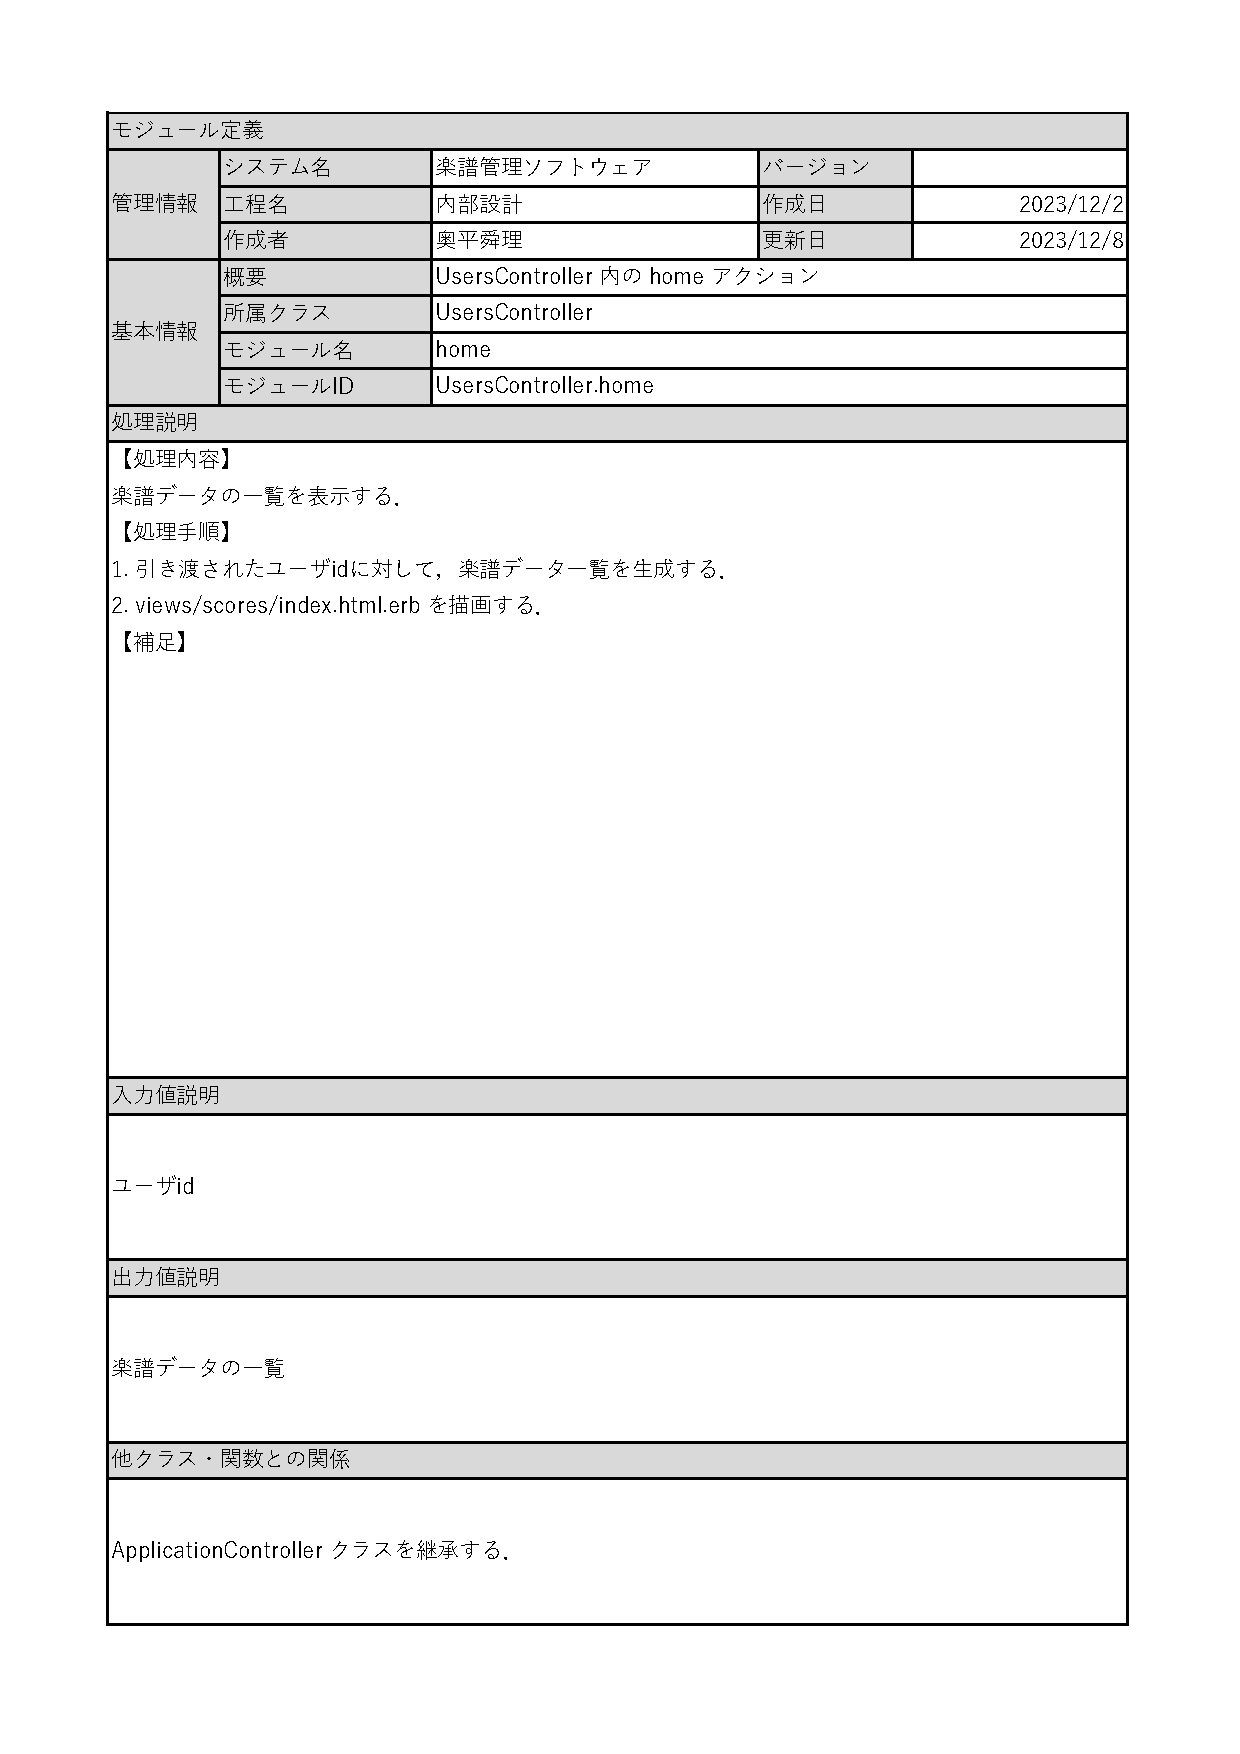
\includegraphics[scale=0.7]{img/Users/xlsx/UsersController_home.pdf}
    \vspace{-1cm}
    \caption{UsersController.home定義書}
\end{figure}
\begin{figure}
    \centering
    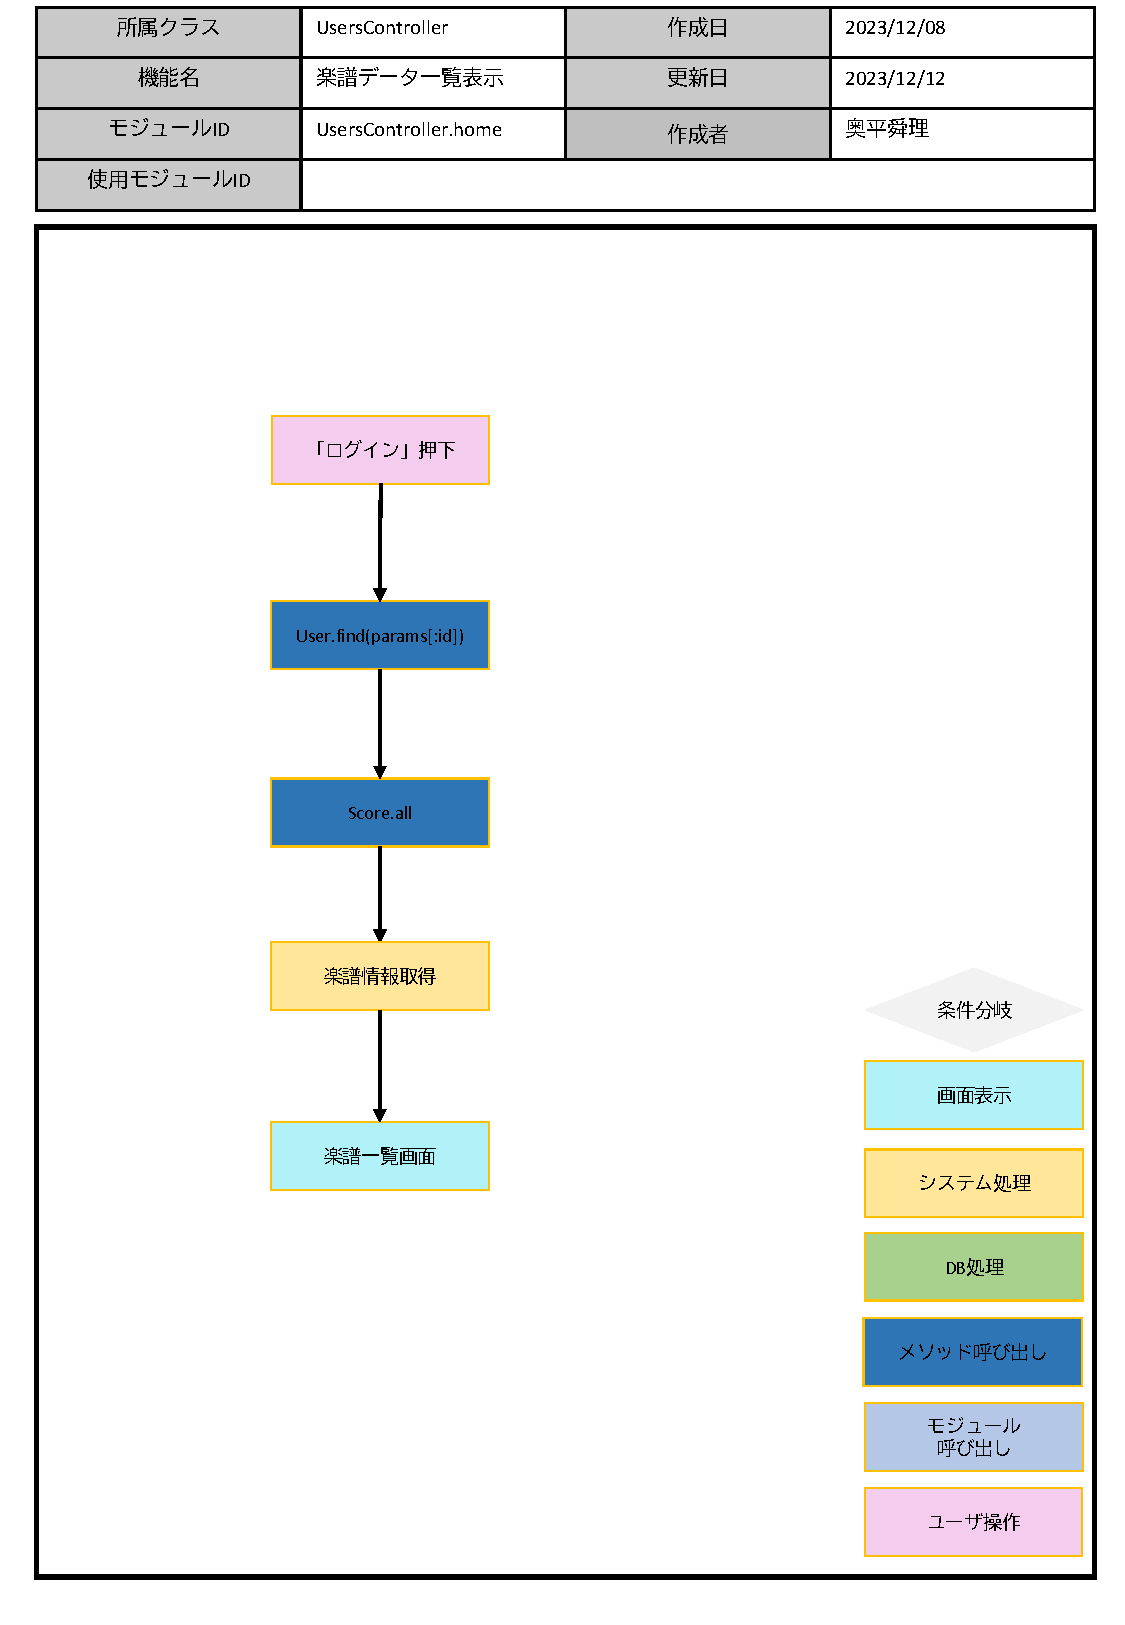
\includegraphics[scale=0.7]{img/Users/pptx/UsersController_home.pdf}
    \caption{UsersController.homeフロー図}
\end{figure}




%show
\begin{figure}
    \centering
    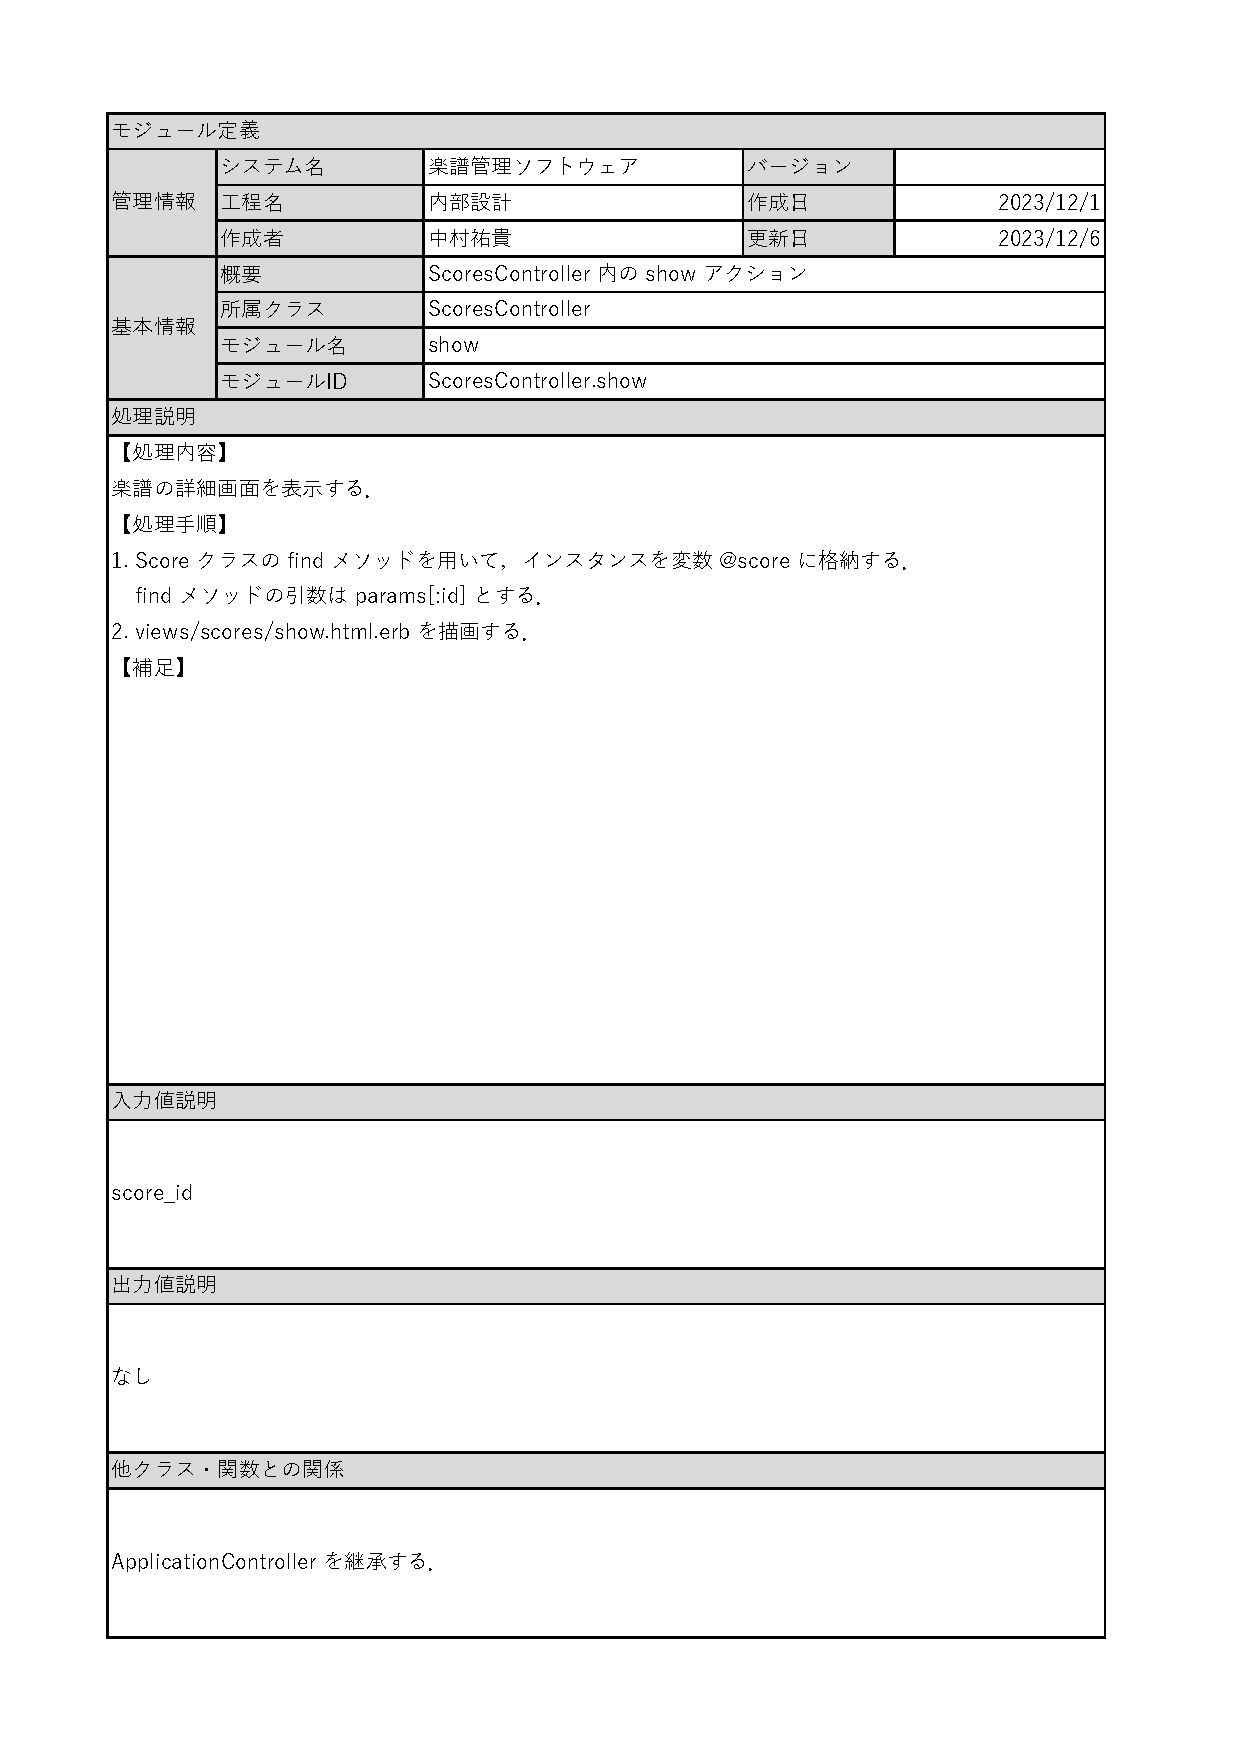
\includegraphics[scale=0.7]{img/Scores/xlsx/ScoresController_show.pdf}
    \vspace{-1cm}
    \caption{ScoresController.show定義書}
\end{figure}
\begin{figure}
    \centering
    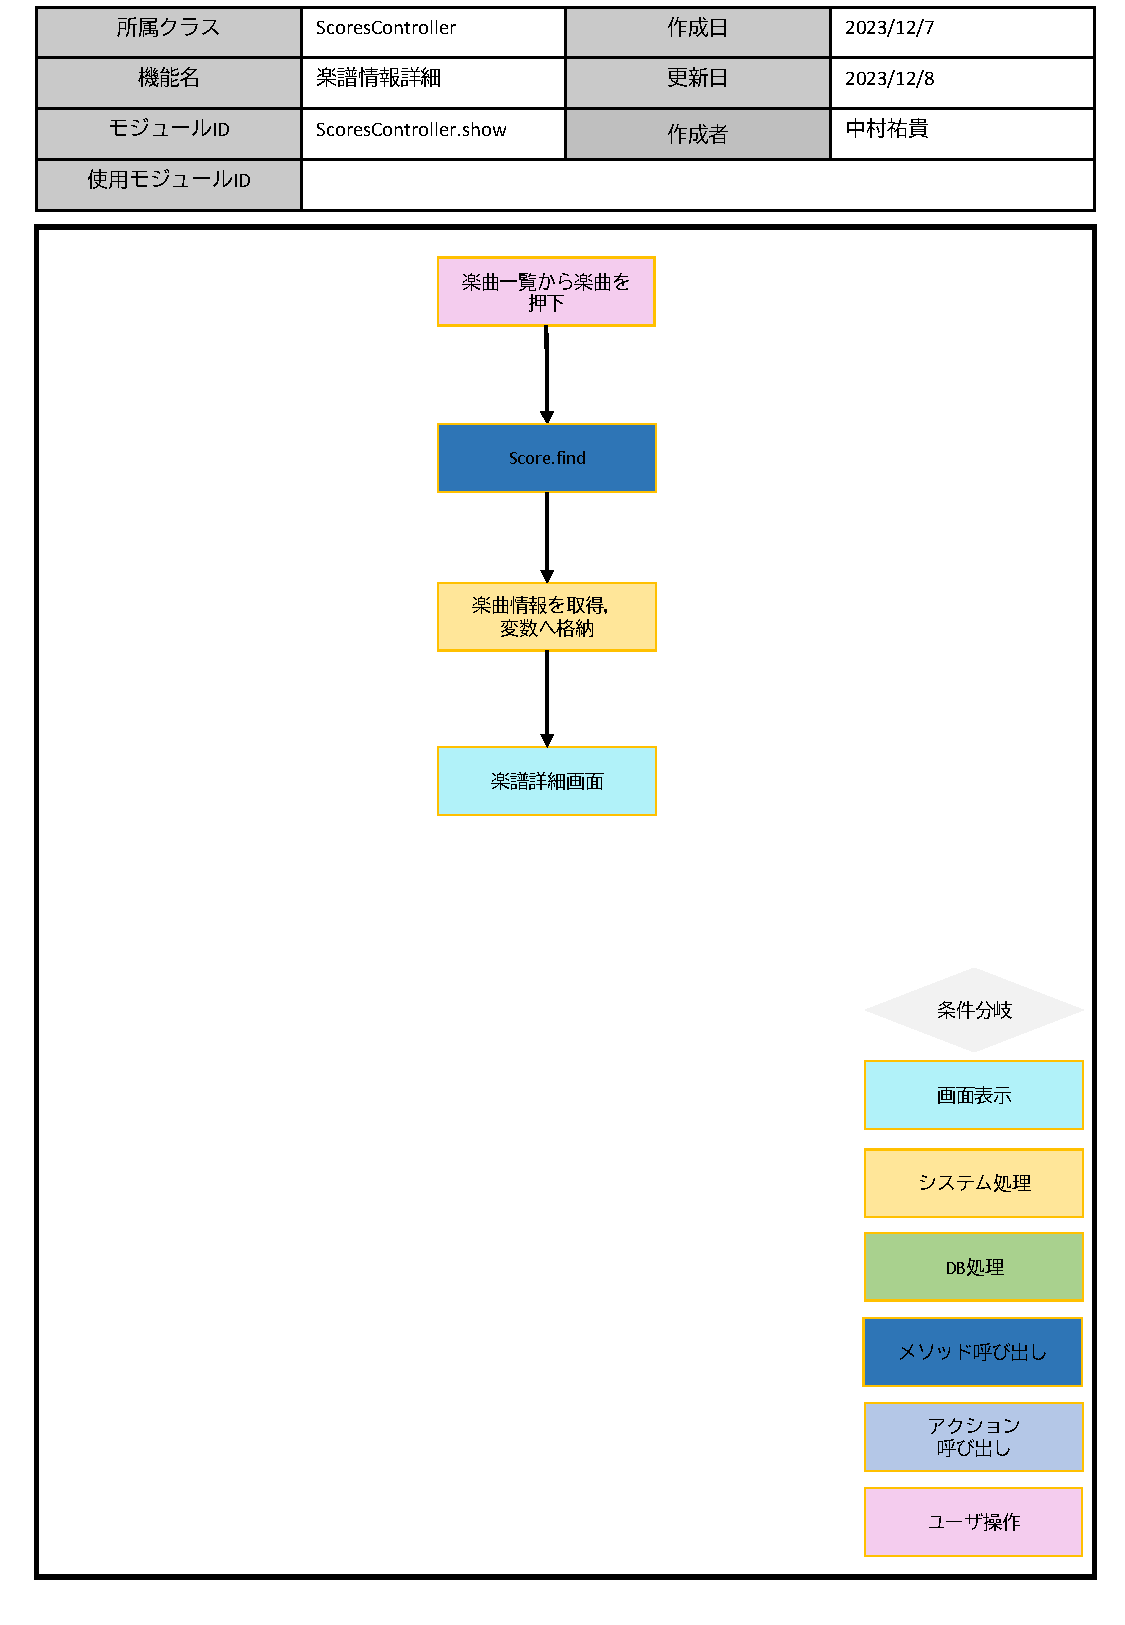
\includegraphics[scale=0.7]{img/Scores/pptx/ScoresController_show.pdf}
    \caption{ScoresController.showフロー図}
\end{figure}
\begin{figure}
    \centering
    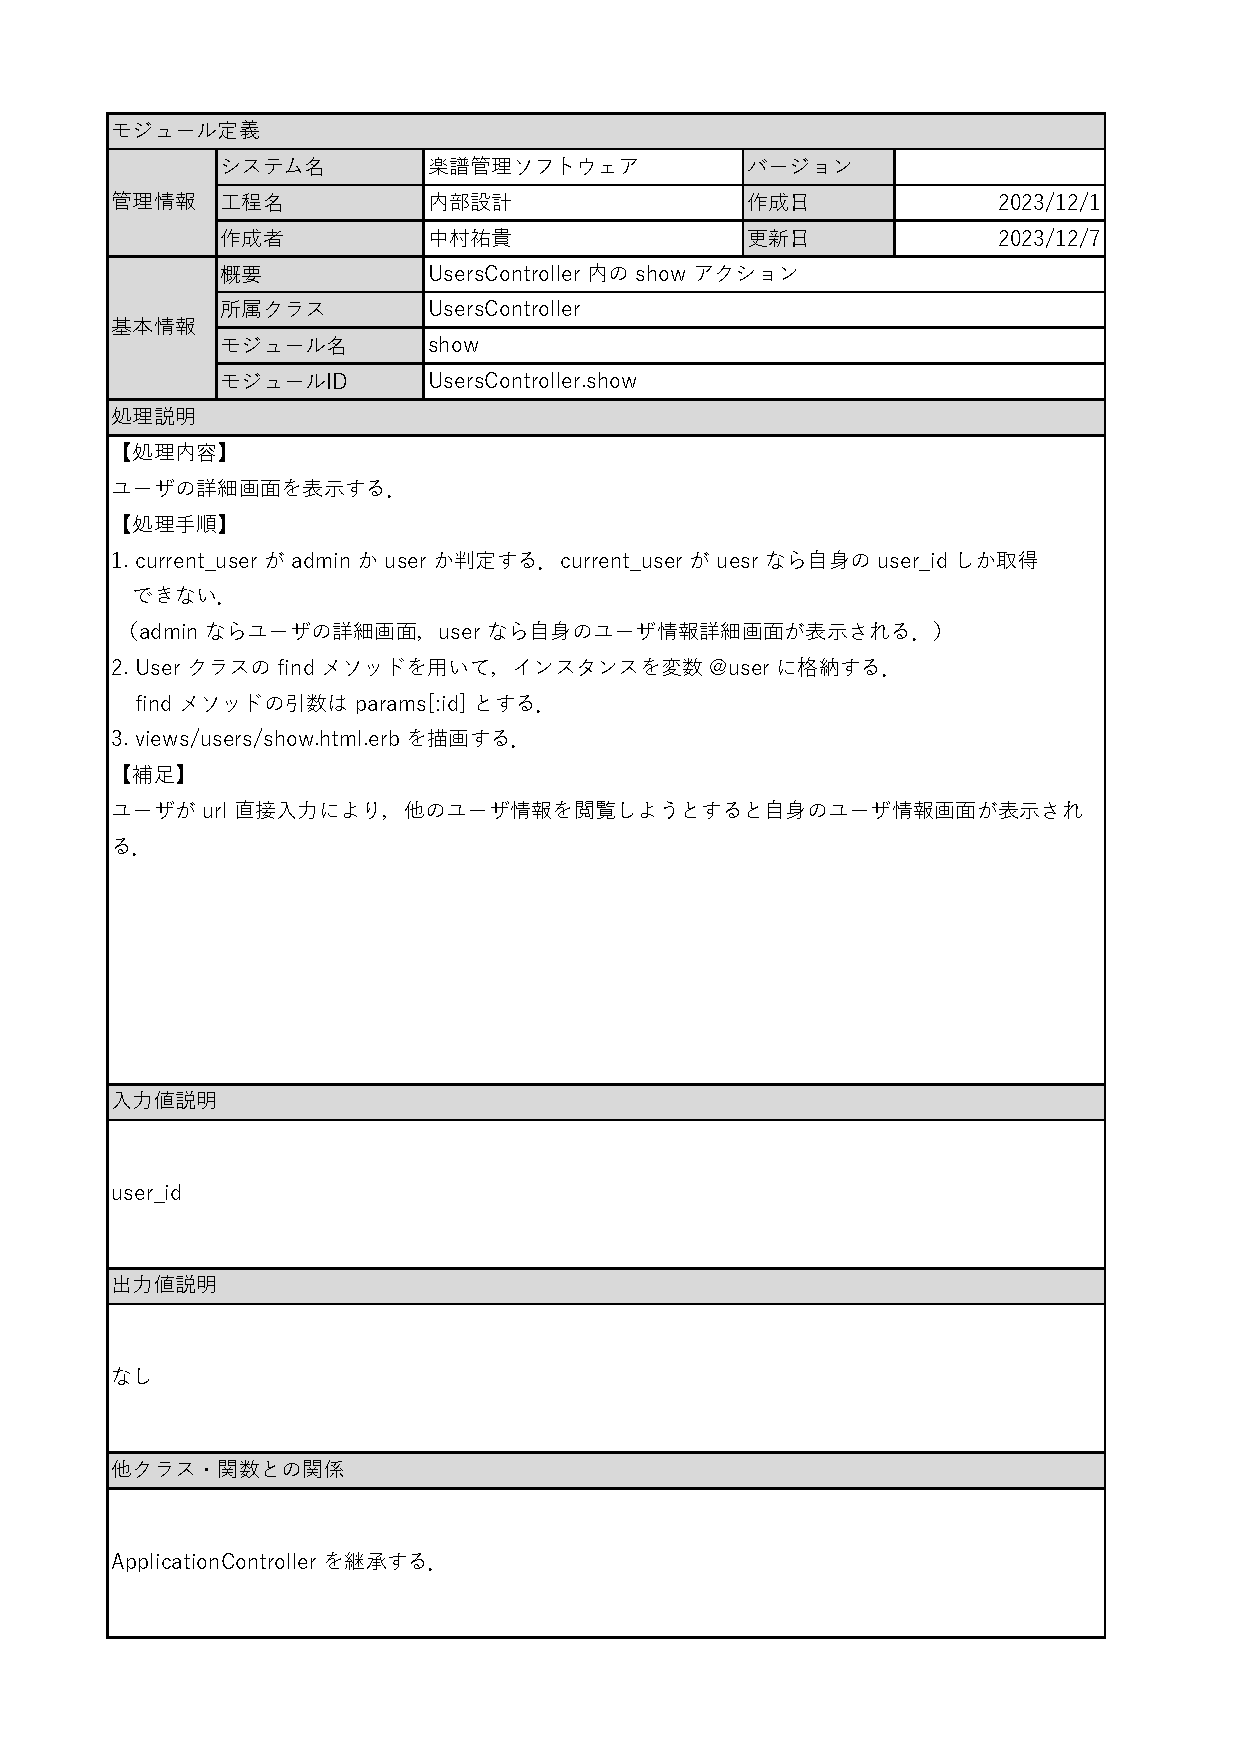
\includegraphics[scale=0.7]{img/Users/xlsx/UsersController_show.pdf}
    \vspace{-0.3cm}
    \caption{UsersController.show定義書}
\end{figure}
\begin{figure}
    \centering
    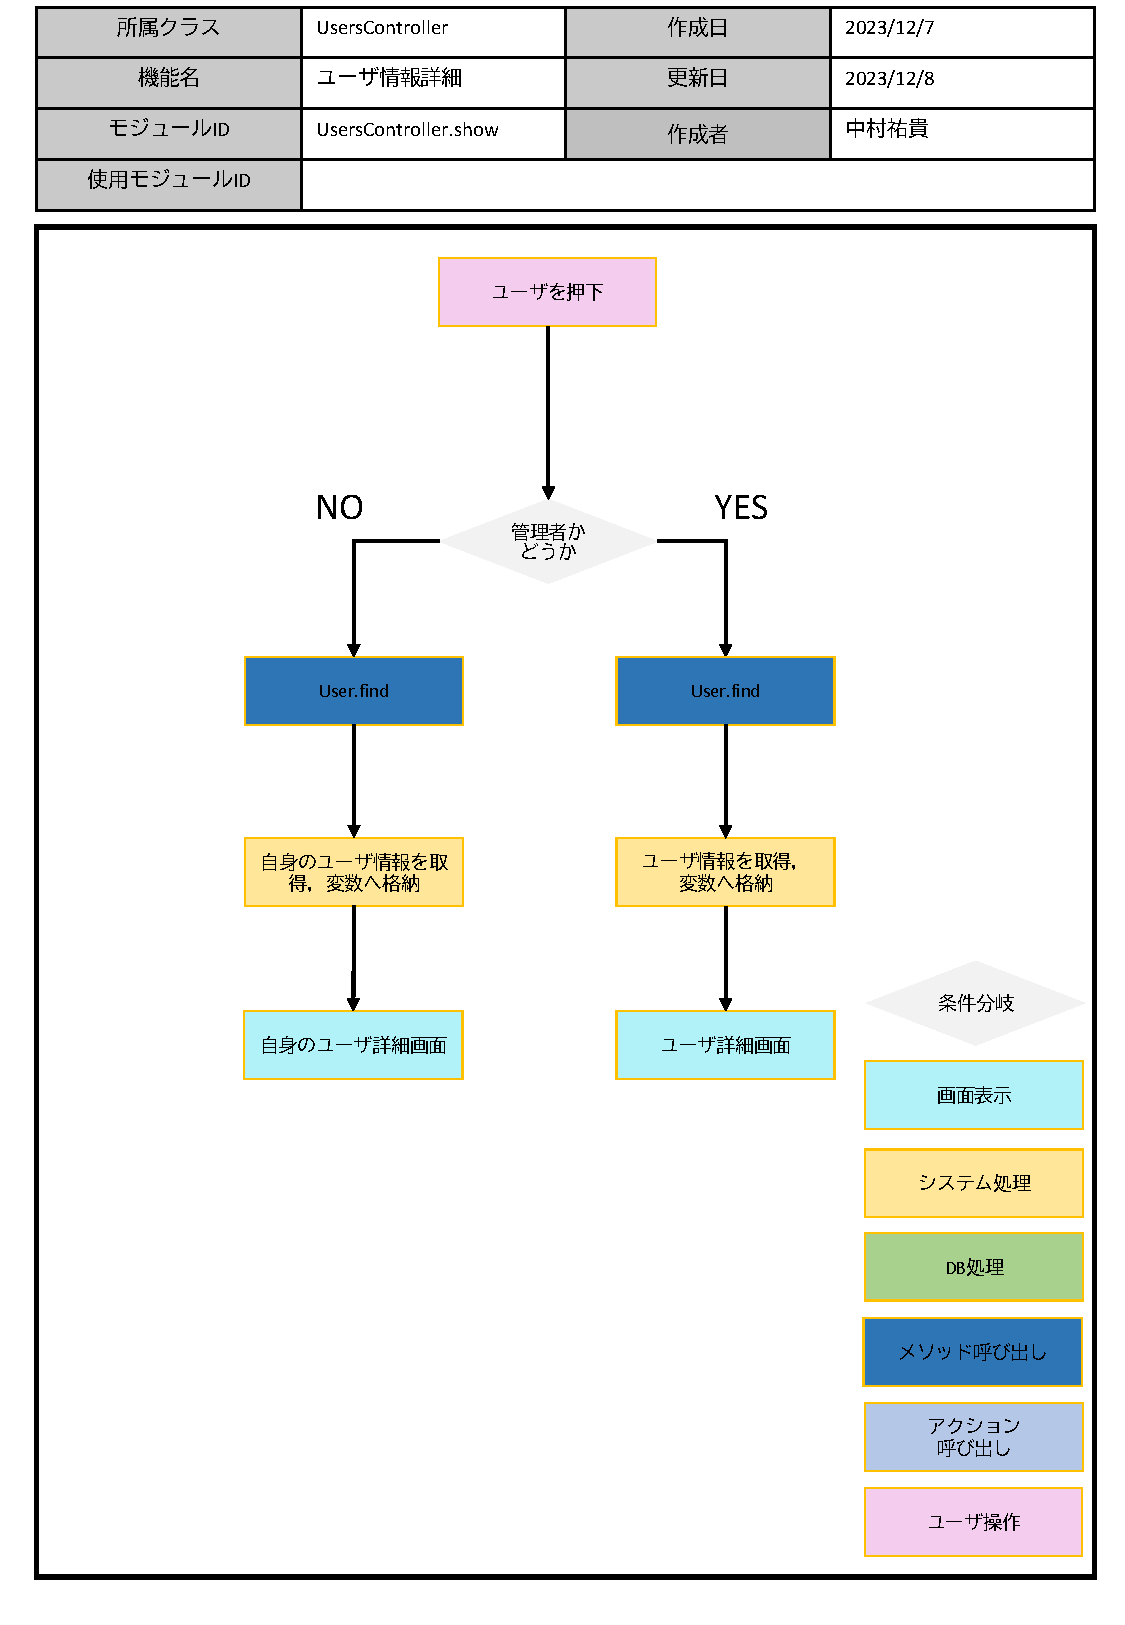
\includegraphics[scale=0.7]{img/Users/pptx/UsersController_show.pdf}
    \vspace{-0.3cm}
    \caption{UsersController.showフロー図}
\end{figure}




%new
\begin{figure}
    \centering
    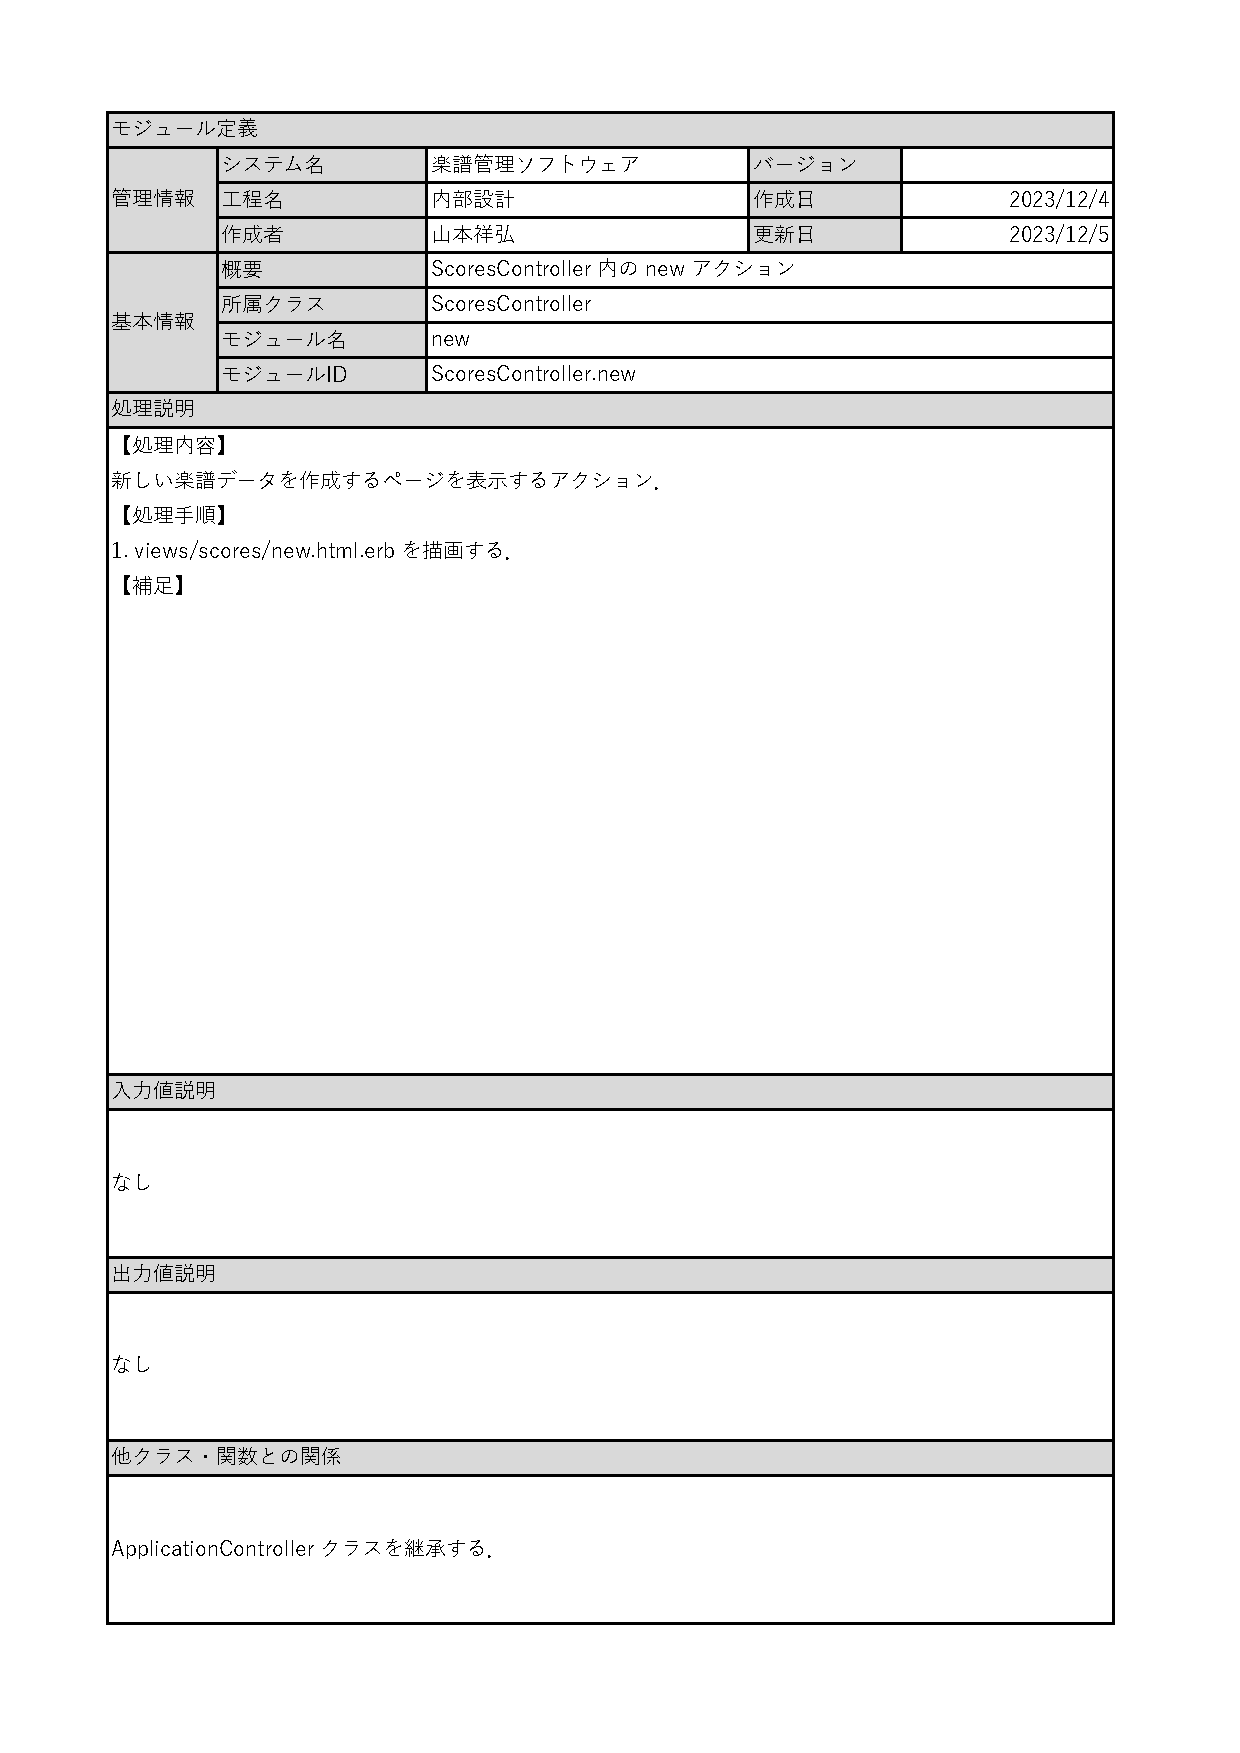
\includegraphics[scale=0.7]{img/Scores/xlsx/ScoresController_new.pdf}
    \vspace{-1cm}
    \caption{ScoresController.new定義書}
\end{figure}
\begin{figure}
    \centering
    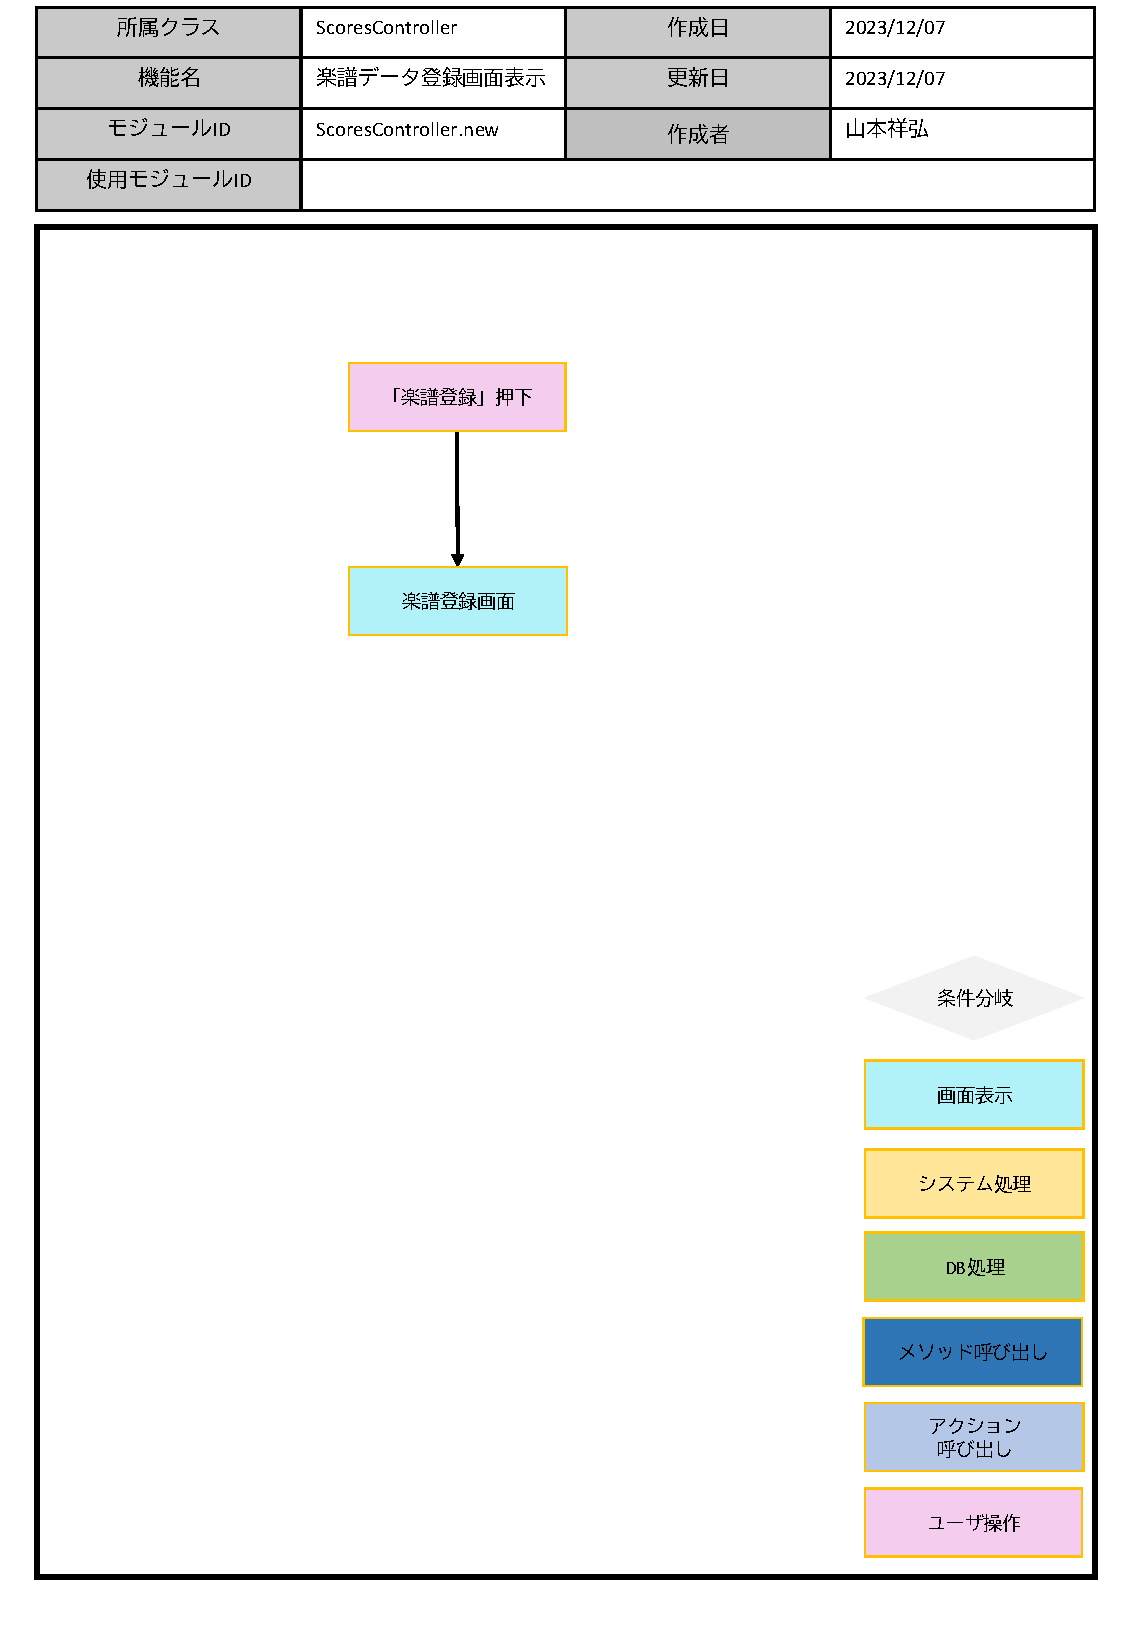
\includegraphics[scale=0.7]{img/Scores/pptx/ScoresController_new.pdf}
    \caption{ScoresController.newフロー図}
\end{figure}
\begin{figure}
    \centering
    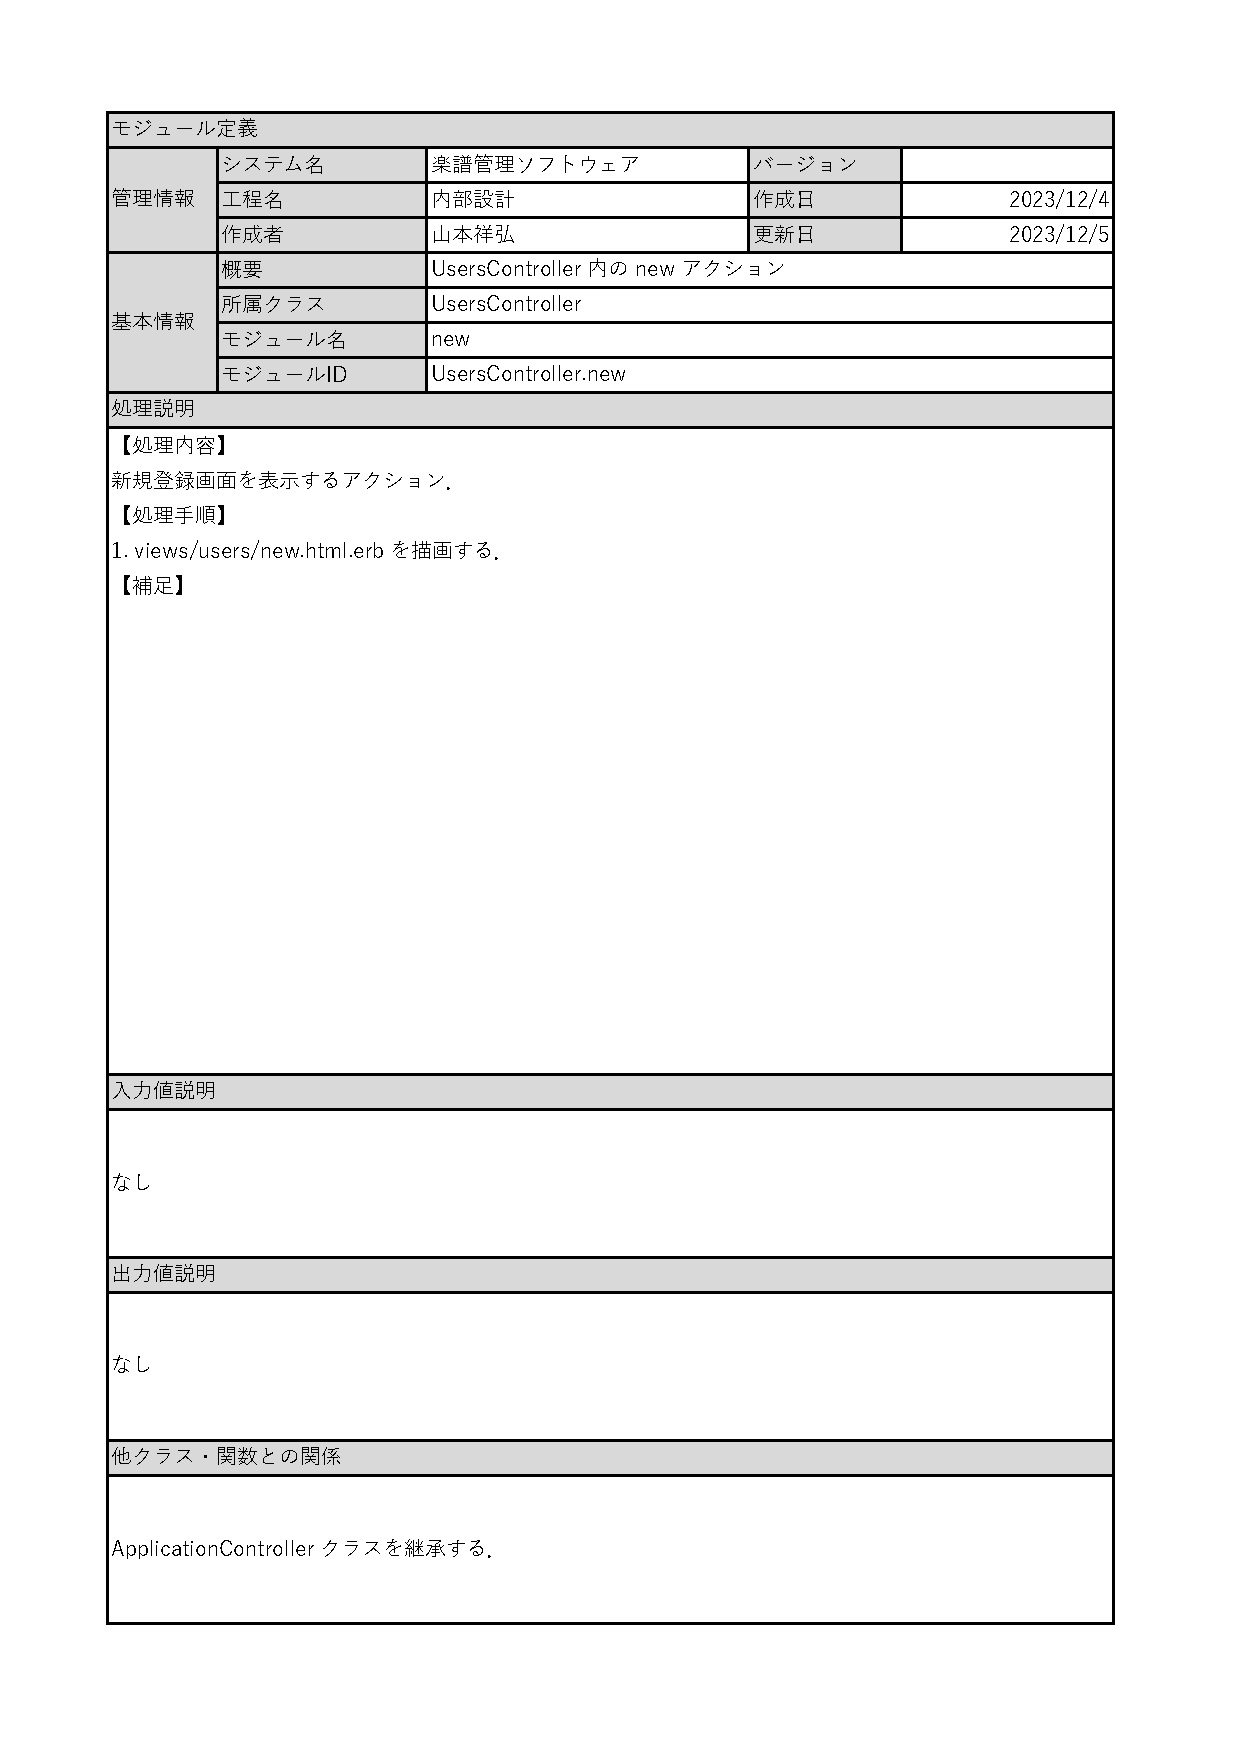
\includegraphics[scale=0.7]{img/Users/xlsx/UsersController_new.pdf}
    \vspace{-1cm}
    \caption{UsersController.new定義書}
\end{figure}
\begin{figure}
    \centering
    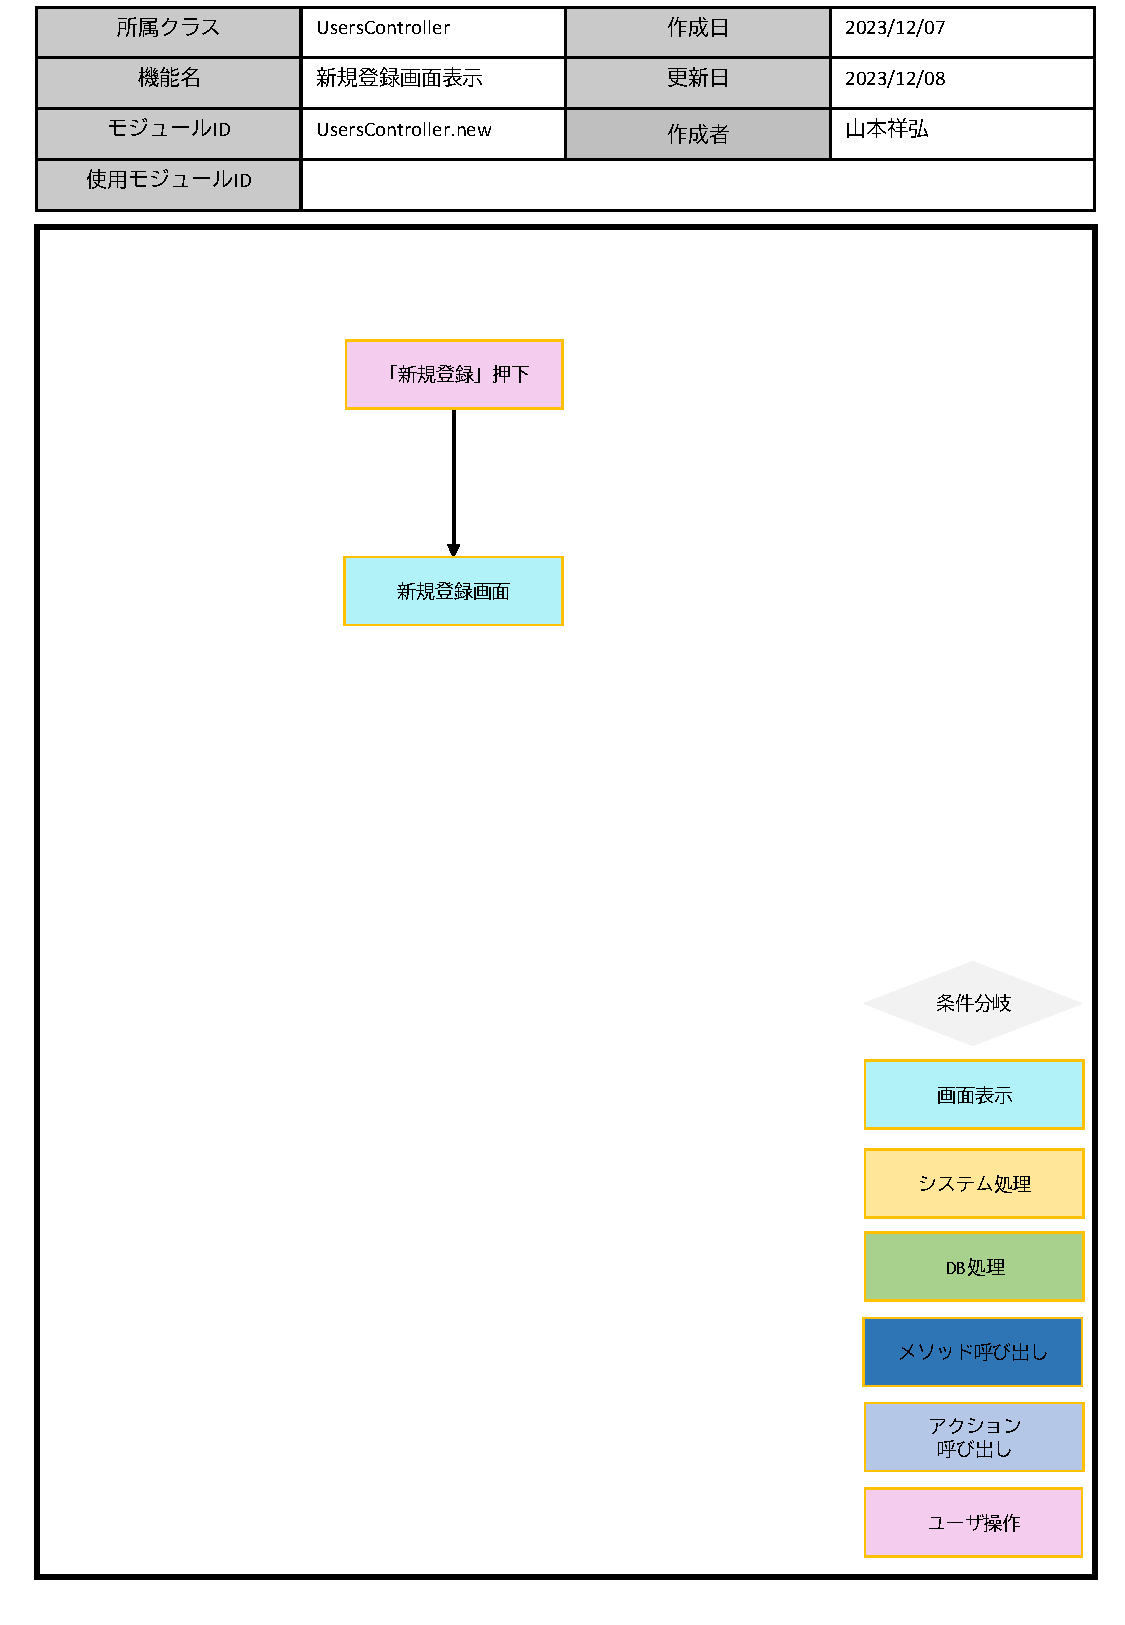
\includegraphics[scale=0.7]{img/Users/pptx/UsersController_new.pdf}
    \caption{UsersController.newフロー図}
\end{figure}




%edit
\begin{figure}
    \centering
    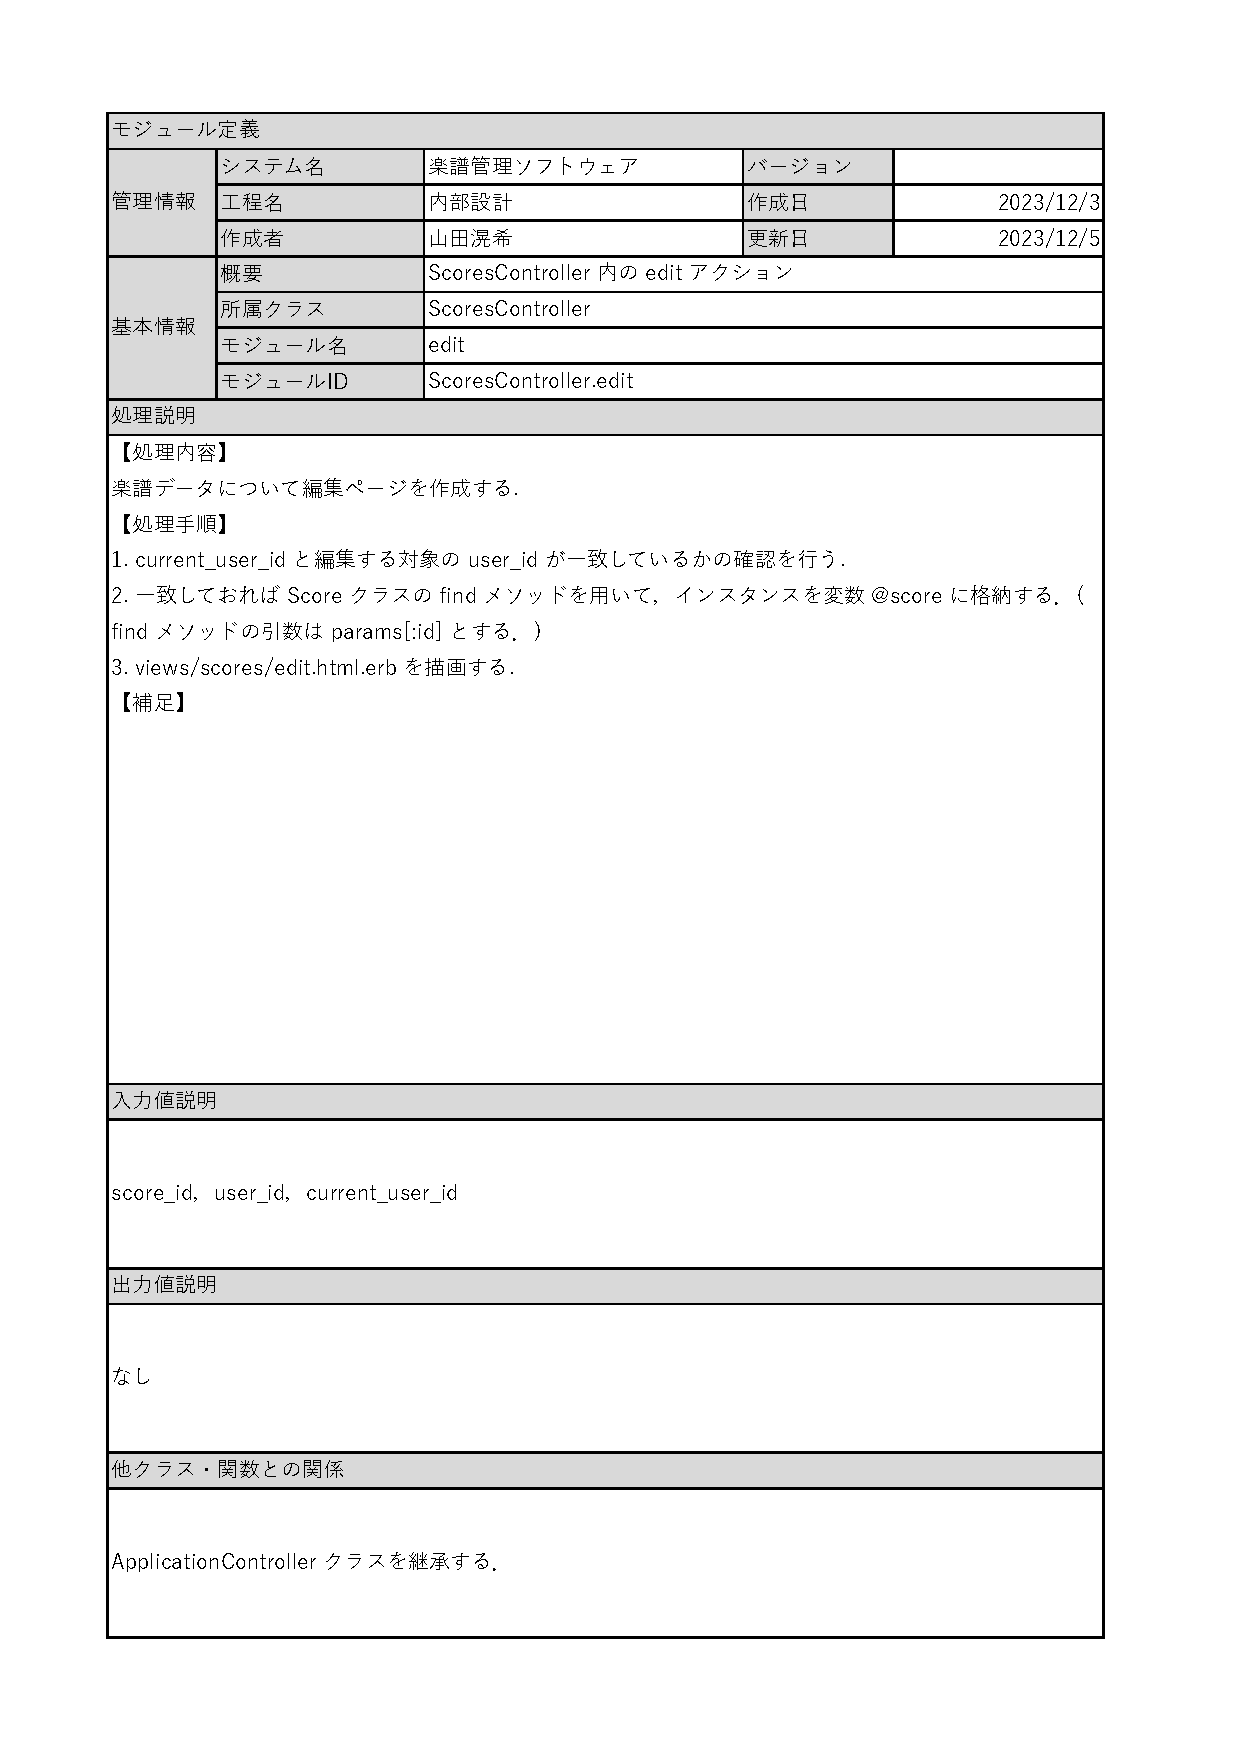
\includegraphics[scale=0.7]{img/Scores/xlsx/ScoresController_edit.pdf}
    \vspace{-1cm}
    \caption{ScoresController.edit定義書}
\end{figure}
\begin{figure}
    \centering
    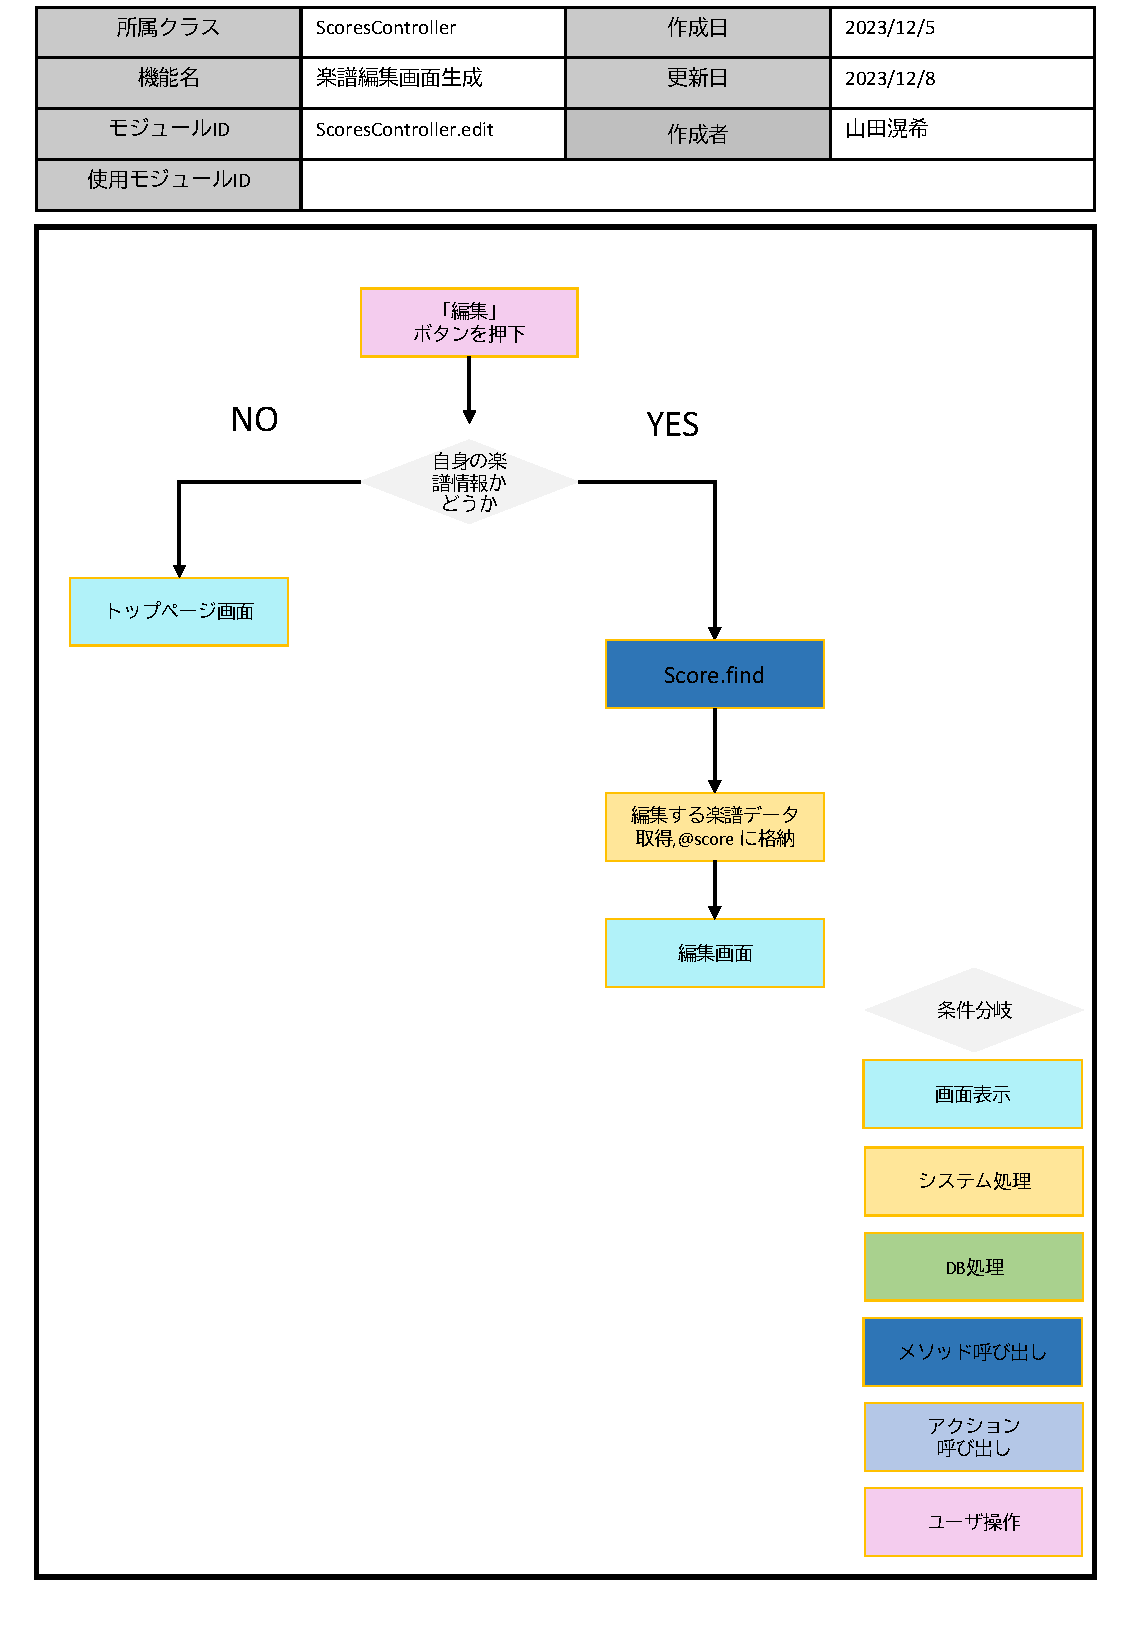
\includegraphics[scale=0.7]{img/Scores/pptx/ScoresController_edit.pdf}
    \caption{ScoresController.editフロー図}
\end{figure}
\begin{figure}
    \centering
    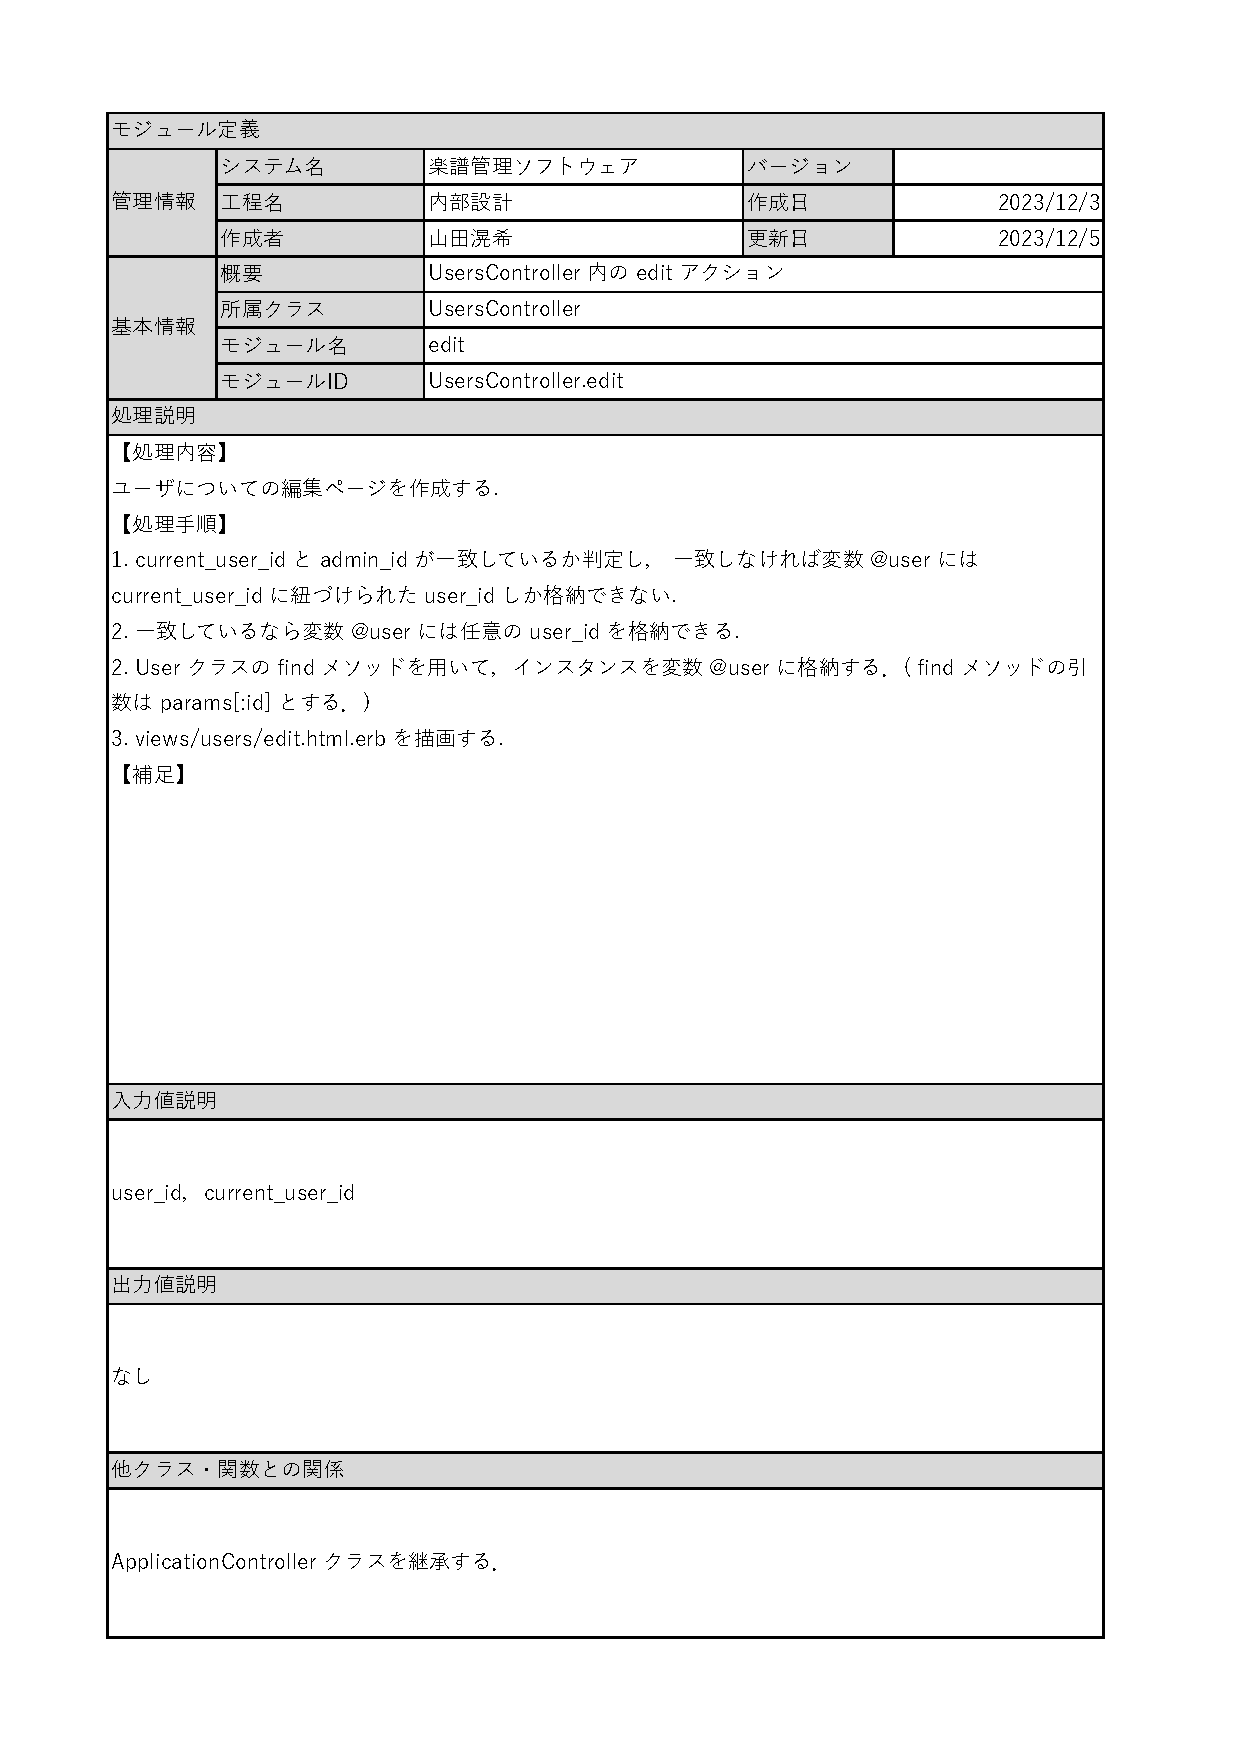
\includegraphics[scale=0.7]{img/Users/xlsx/UsersController_edit.pdf}
    \vspace{-1cm}
    \caption{UsersController.edit定義書}
\end{figure}
\begin{figure}
    \centering
    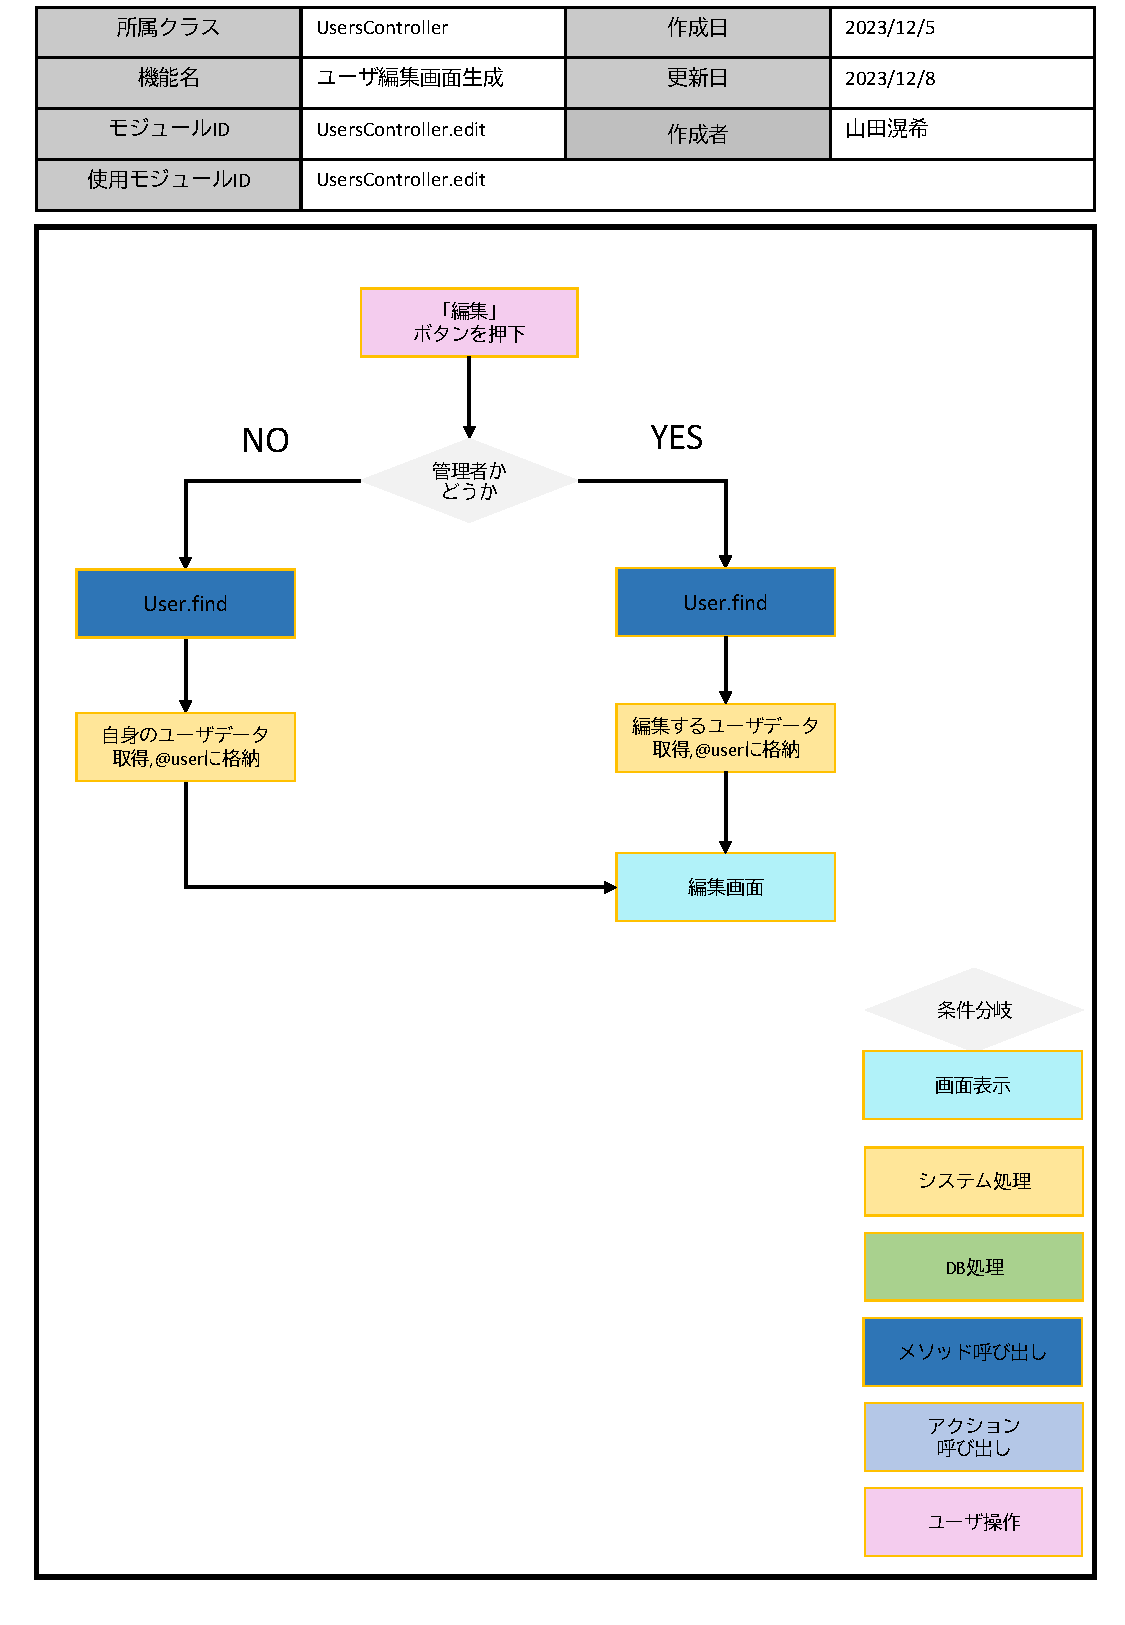
\includegraphics[scale=0.7]{img/Users/pptx/UsersController_edit.pdf}
    \caption{UsersController.editフロー図}
\end{figure}




%create
\begin{figure}[h]
    \centering
    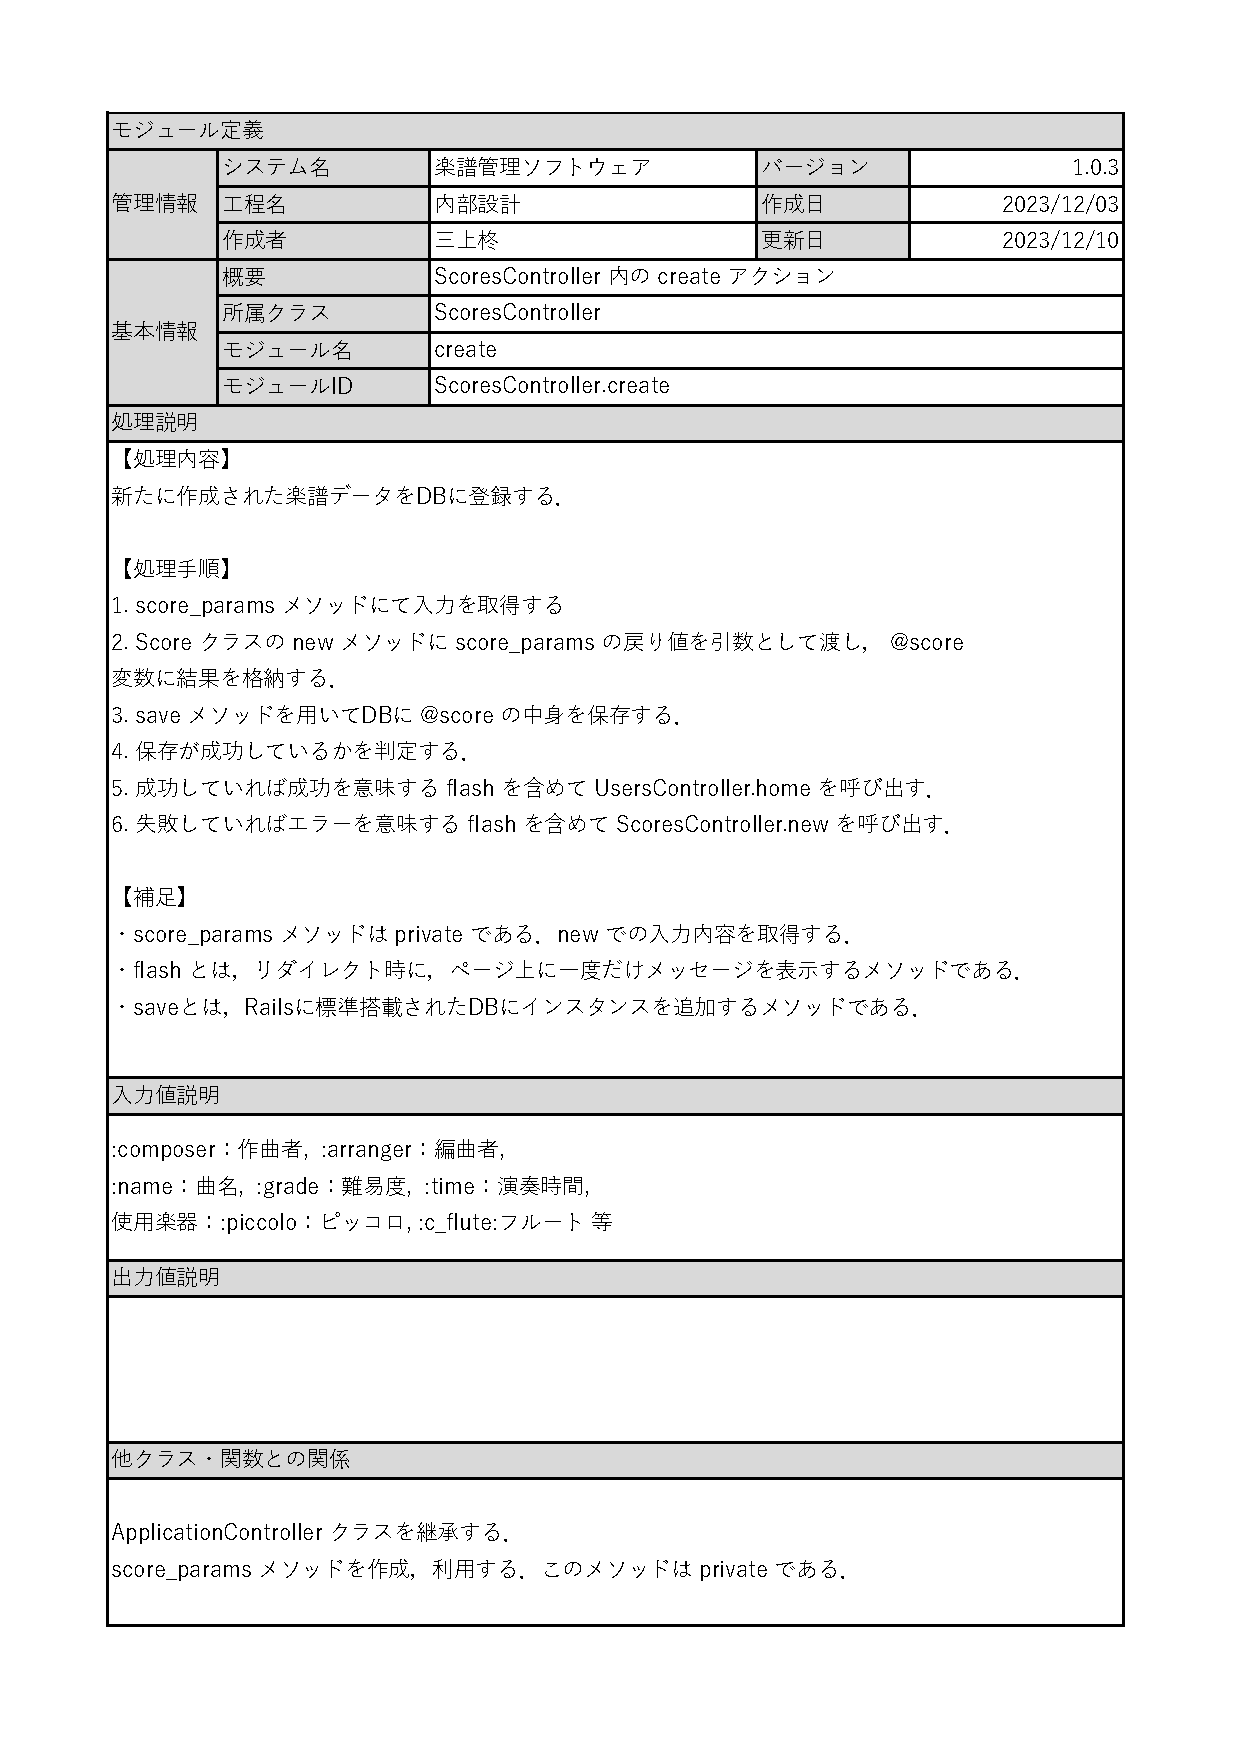
\includegraphics[scale=0.7]{img/Scores/xlsx/ScoresController_create.pdf}
    \vspace{-1cm}
    \caption{ScoresController.create定義書}
\end{figure}
\begin{figure}
    \centering
    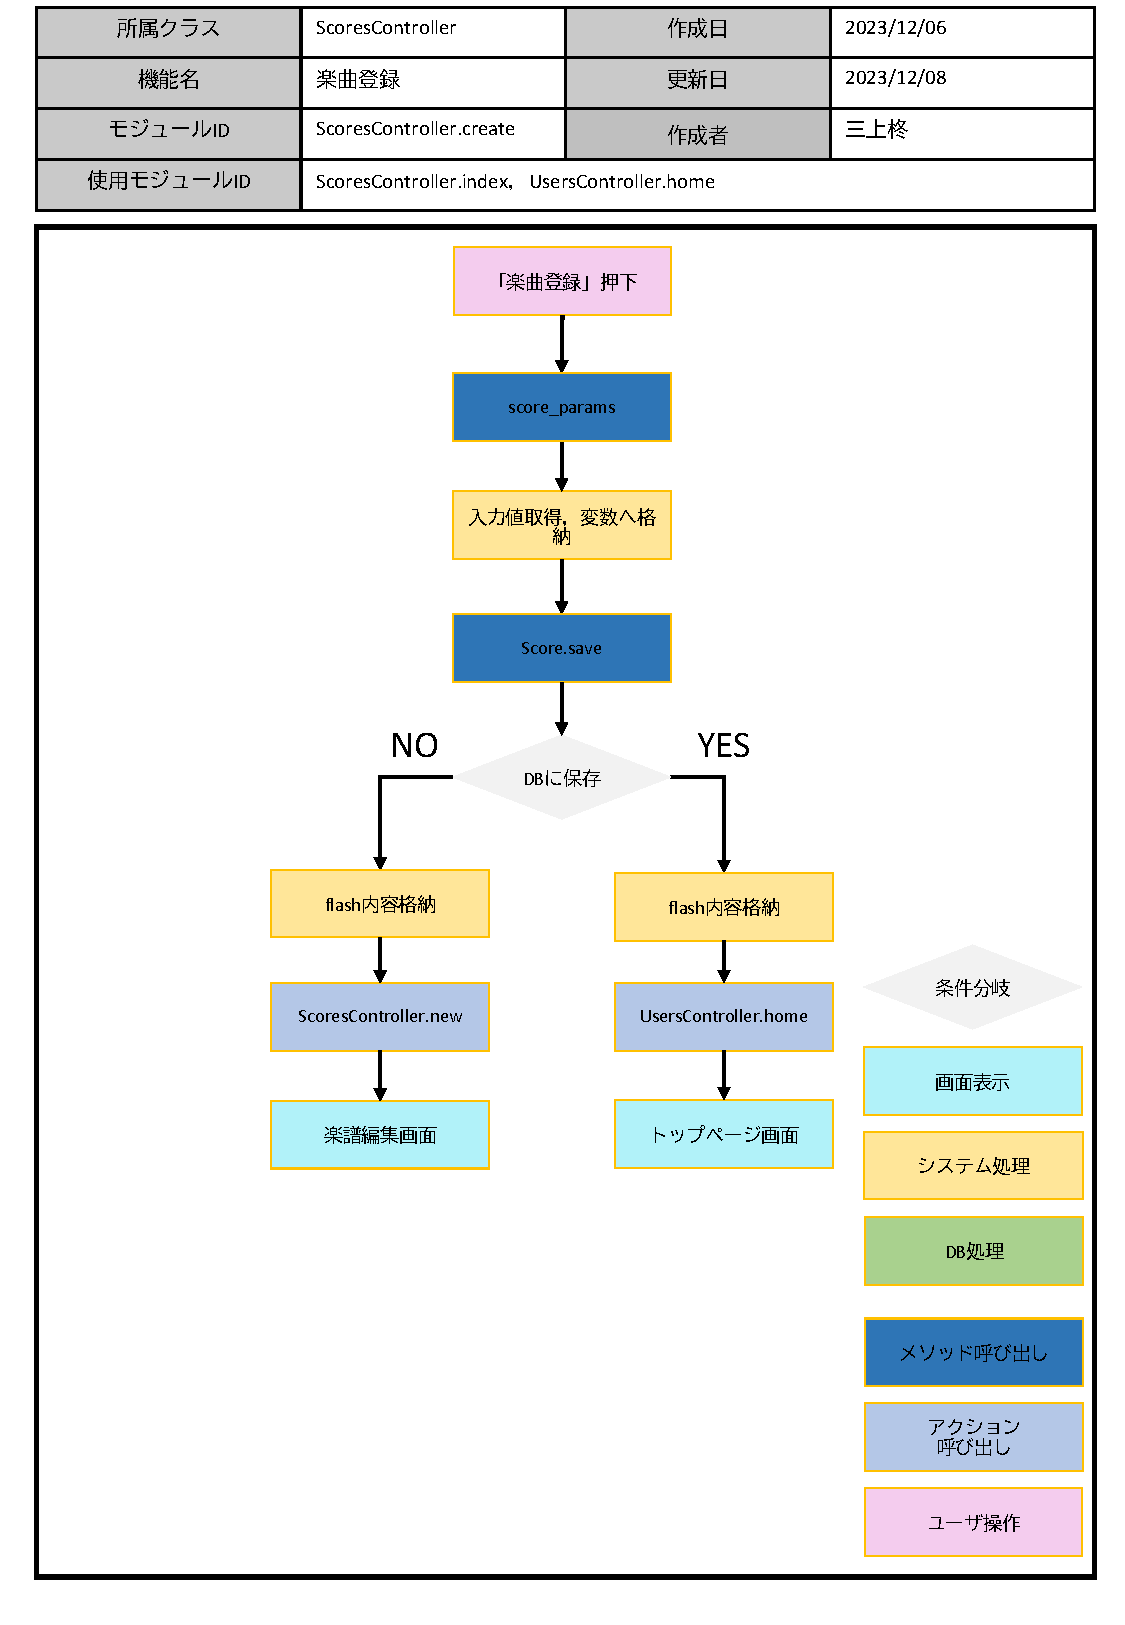
\includegraphics[scale=0.7]{img/Scores/pptx/ScoresController_create.pdf}
    \caption{ScoresController.createフロー図}
\end{figure}
\begin{figure}
    \centering
    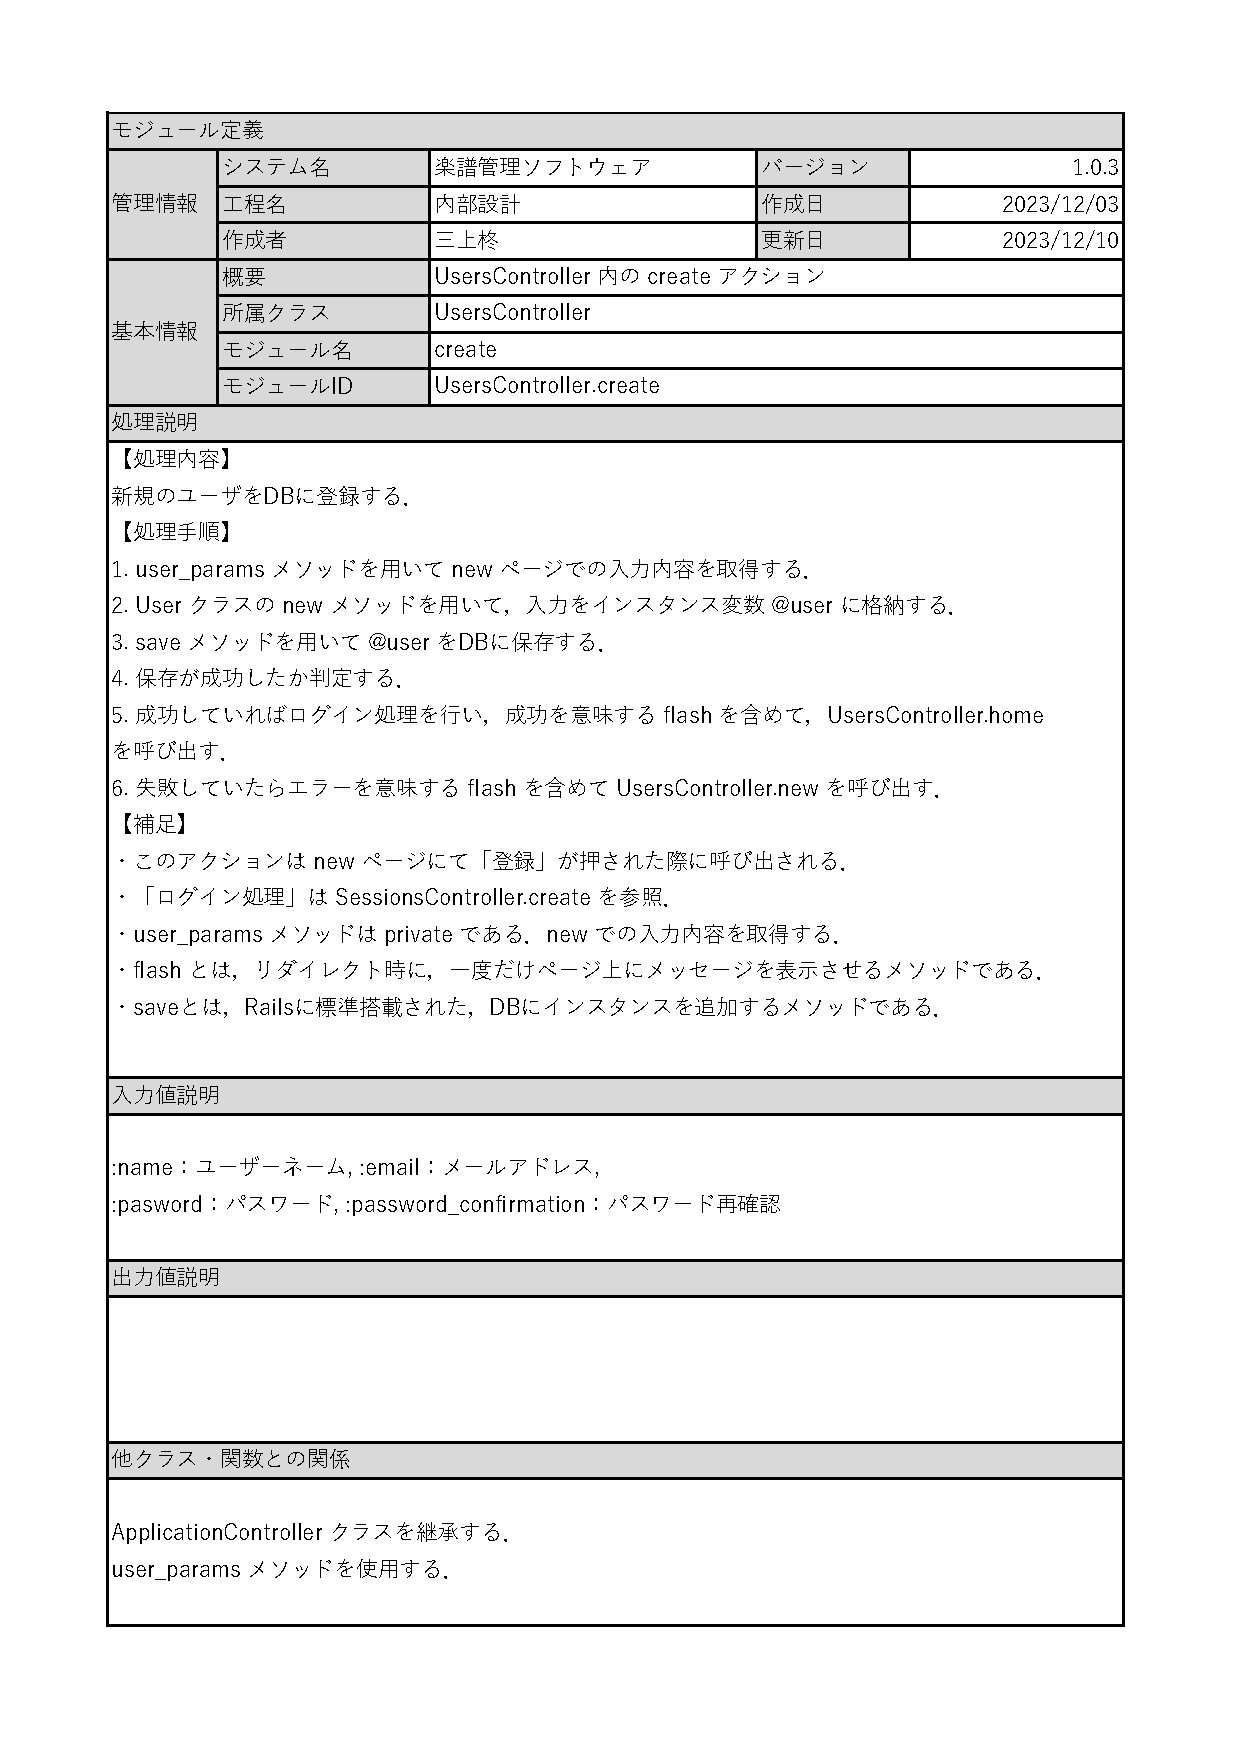
\includegraphics[scale=0.7]{img/Users/xlsx/UsersController_create.pdf}
    \vspace{-1cm}
    \caption{UsersController.create定義書}
\end{figure}
\begin{figure}
    \centering
    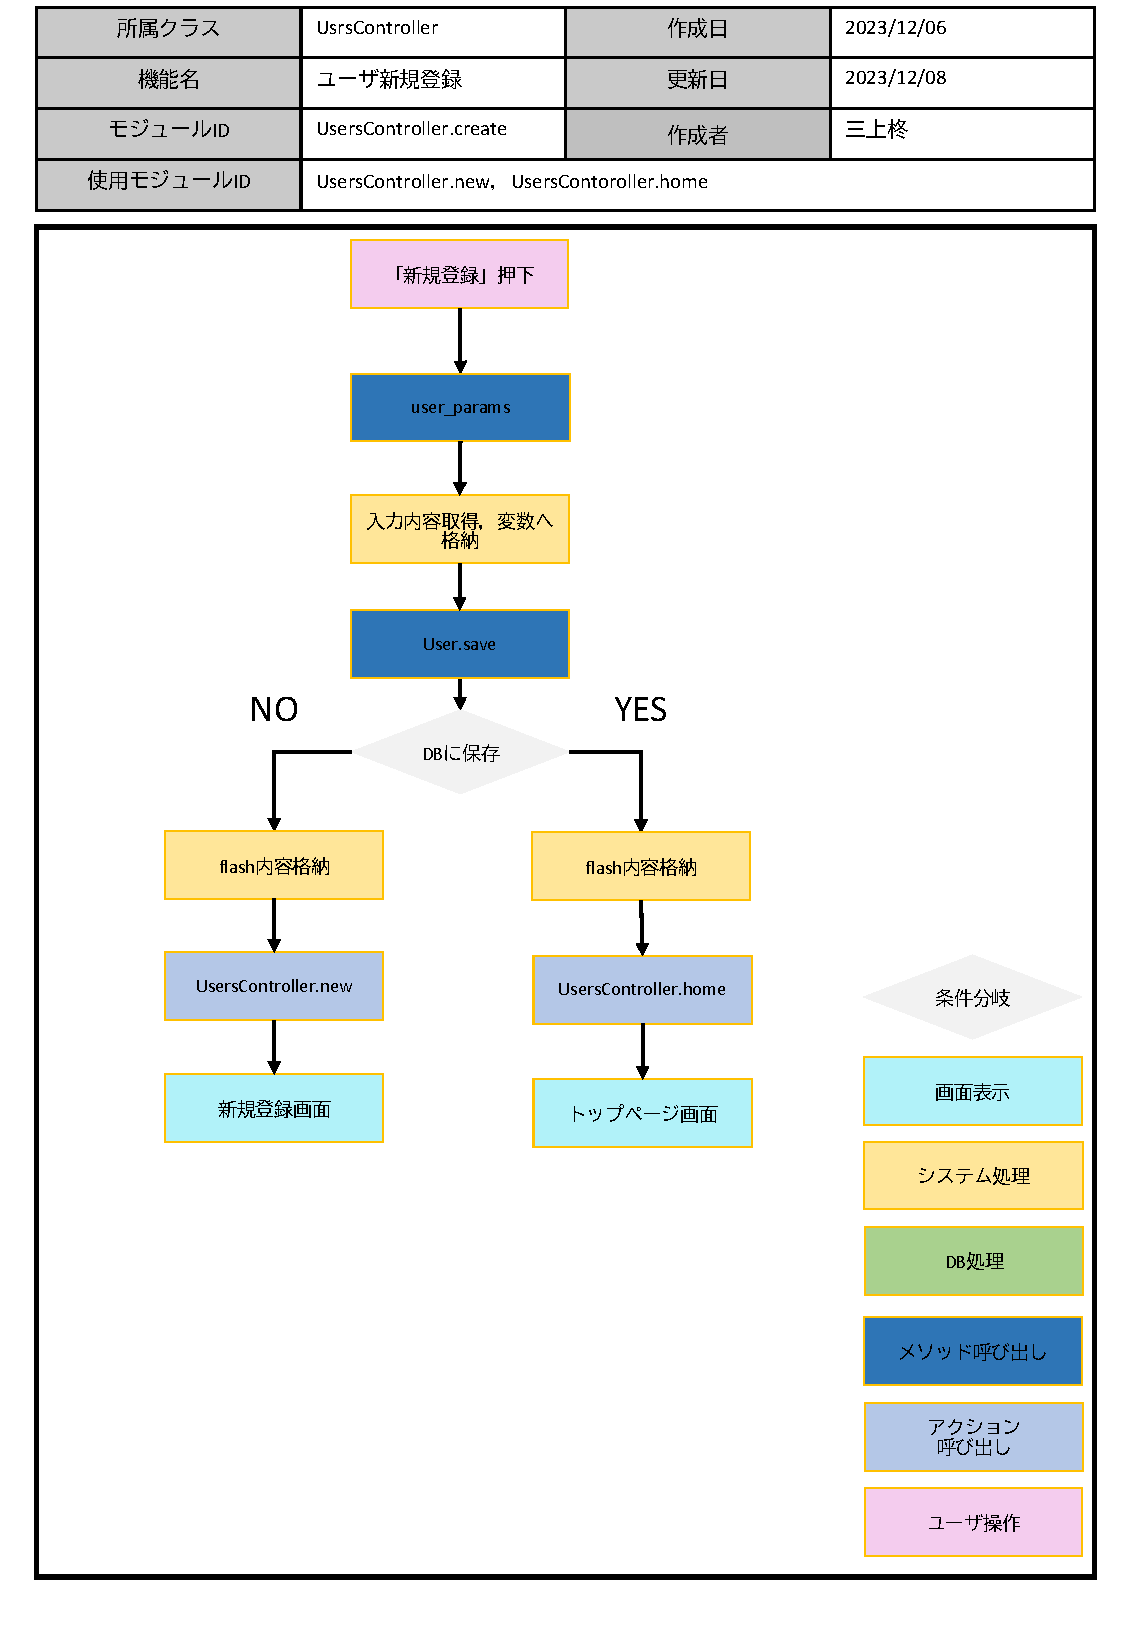
\includegraphics[scale=0.7]{img/Users/pptx/UsersController_create.pdf}
    \caption{UsersController.createフロー図}
\end{figure}

%create
\begin{figure}[h]
    \centering
    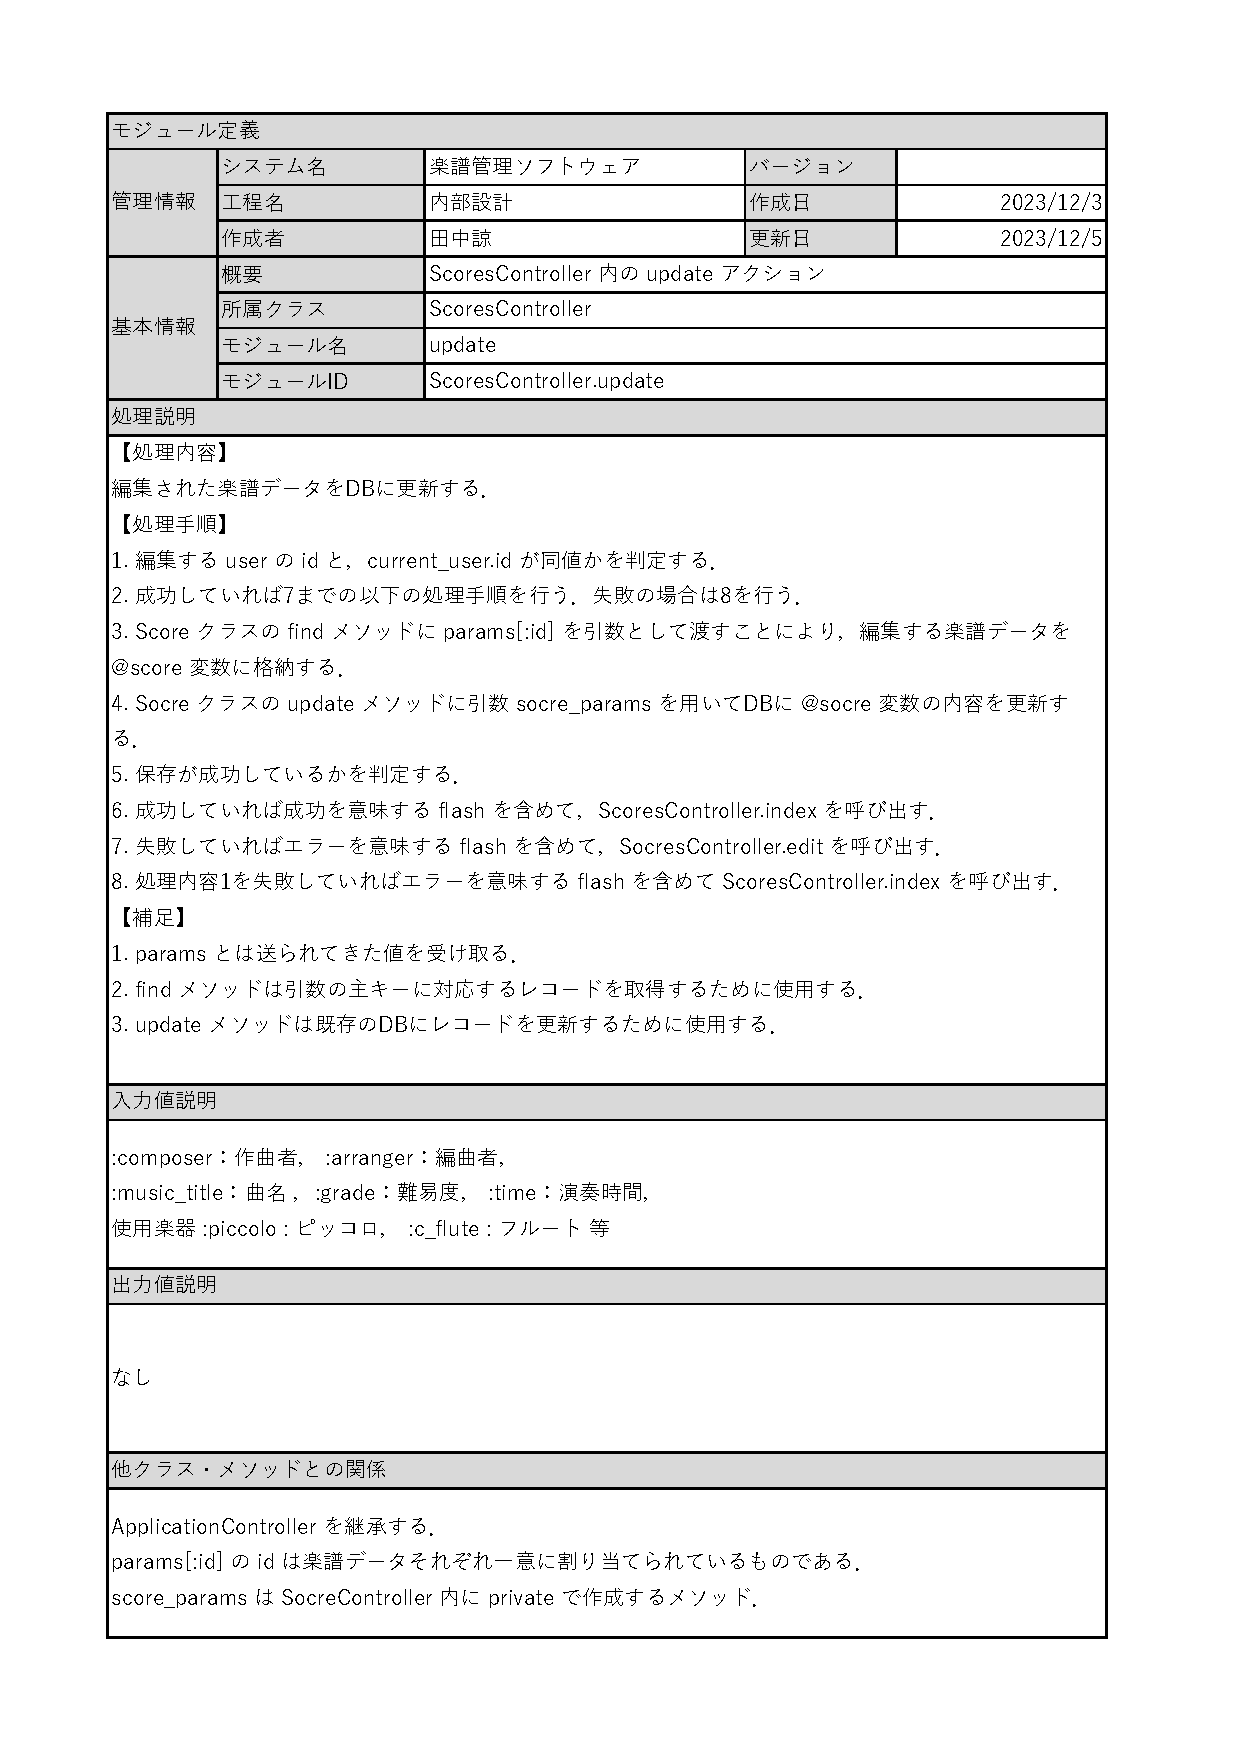
\includegraphics[scale=0.7]{img/Scores/xlsx/ScoresController_update.pdf}
    \vspace{-1cm}
    \caption{ScoresController.update定義書}
\end{figure}
\begin{figure}
    \centering
    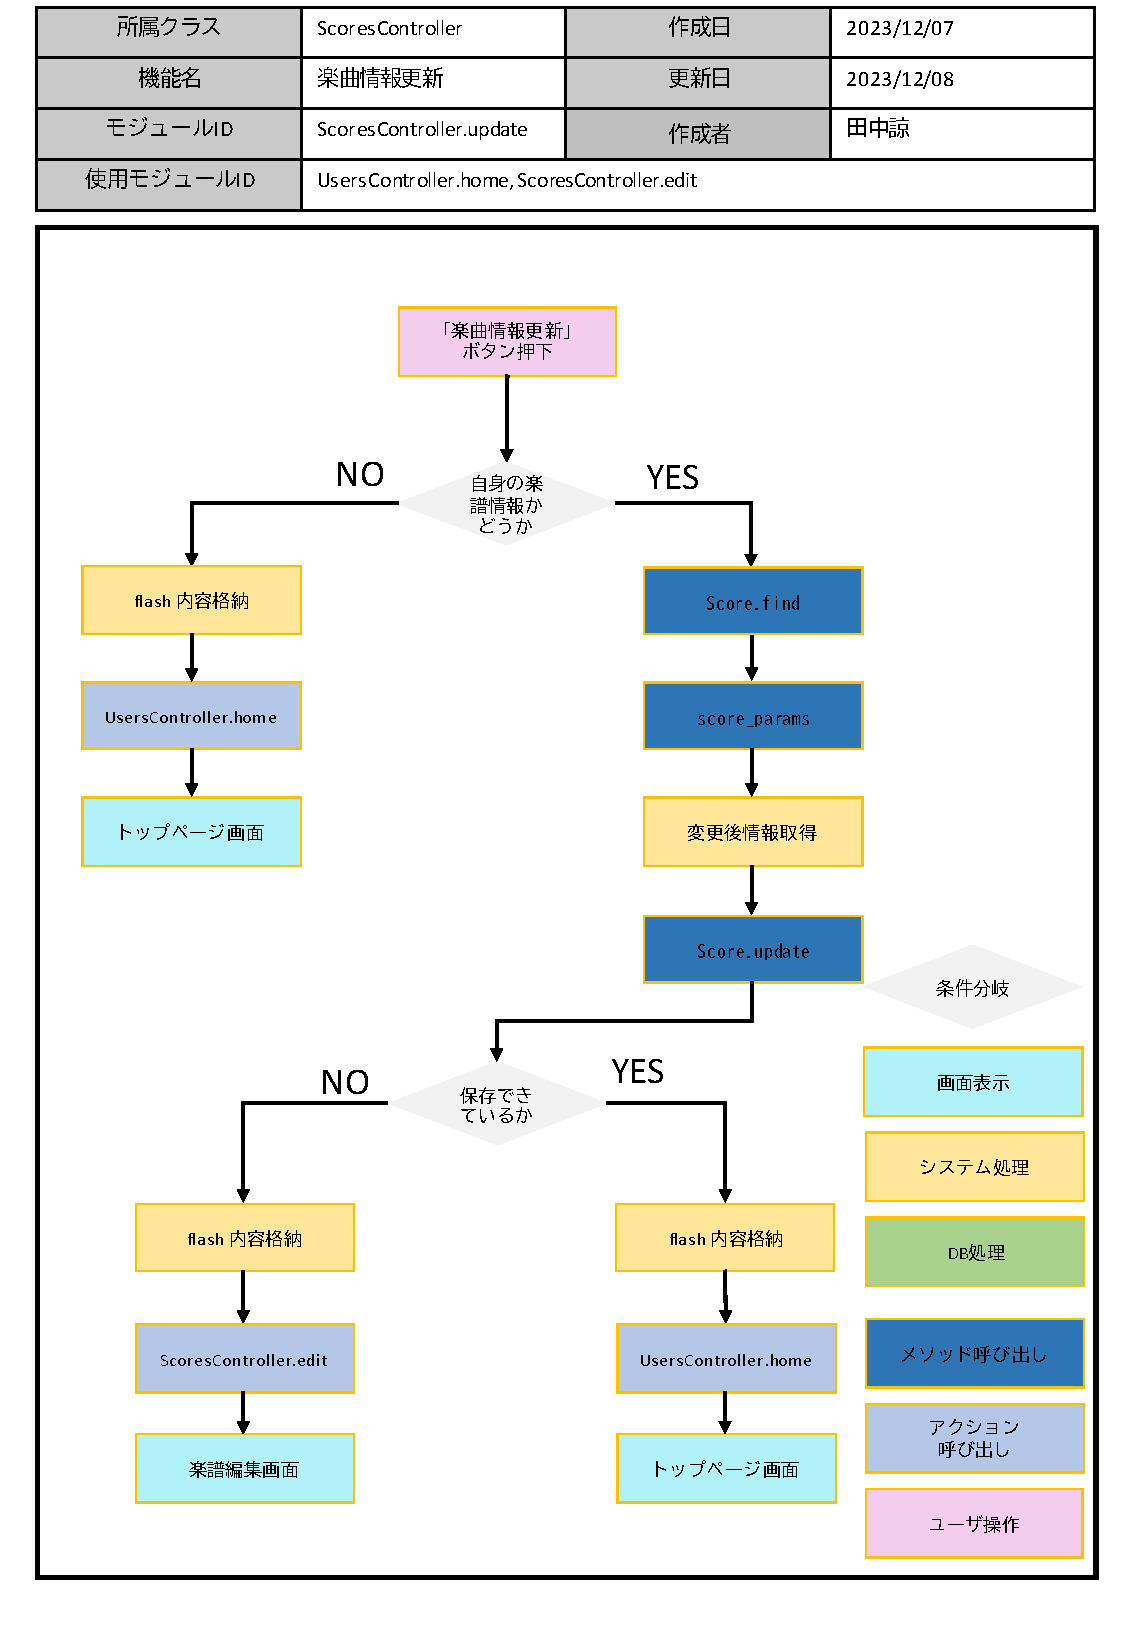
\includegraphics[scale=0.7]{img/Scores/pptx/ScoresController_update.pdf}
    \caption{ScoresController.updateフロー図}
\end{figure}
\begin{figure}
    \centering
    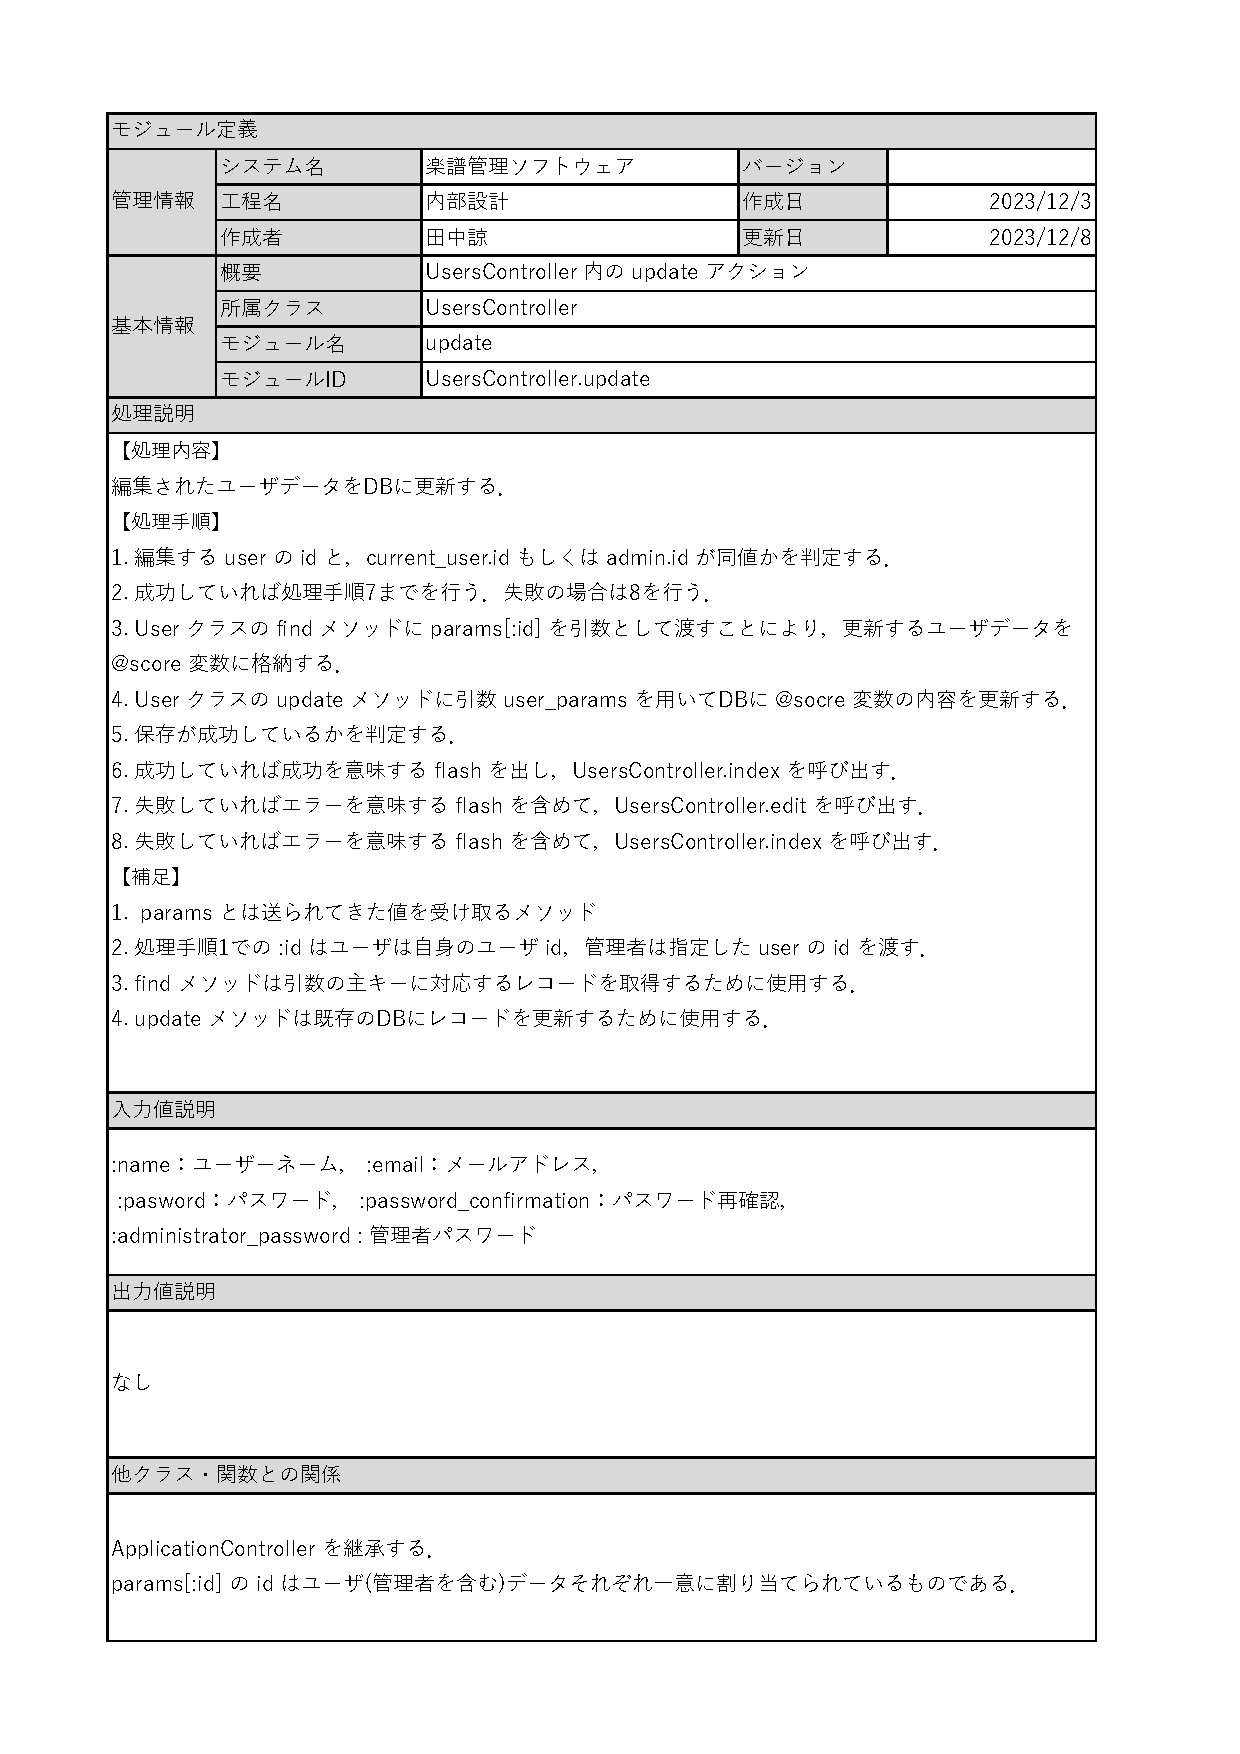
\includegraphics[scale=0.7]{img/Users/xlsx/UsersController_update.pdf}
    \vspace{-1cm}
    \caption{UsersController.update定義書}
\end{figure}
\begin{figure}
    \centering
    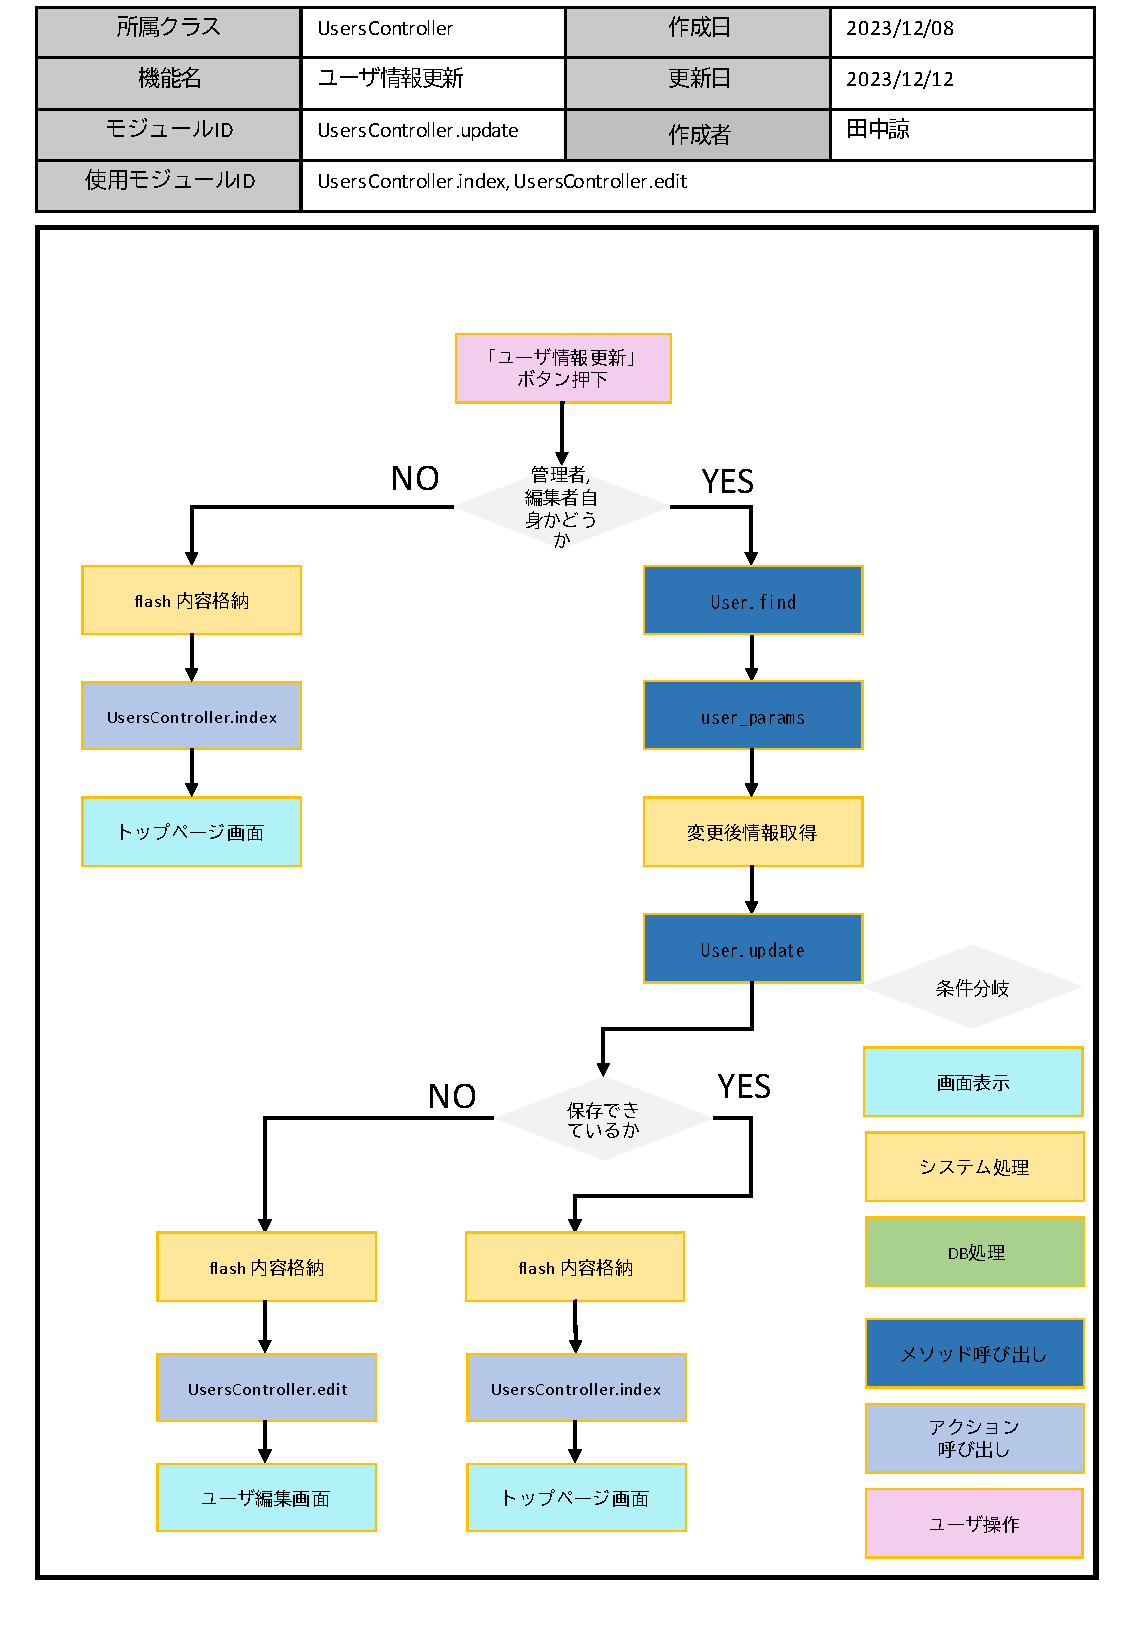
\includegraphics[scale=0.7]{img/Users/pptx/UsersController_update.pdf}
    \caption{UsersController.updateフロー図}
\end{figure}


%destroy
\begin{figure}
    \centering
    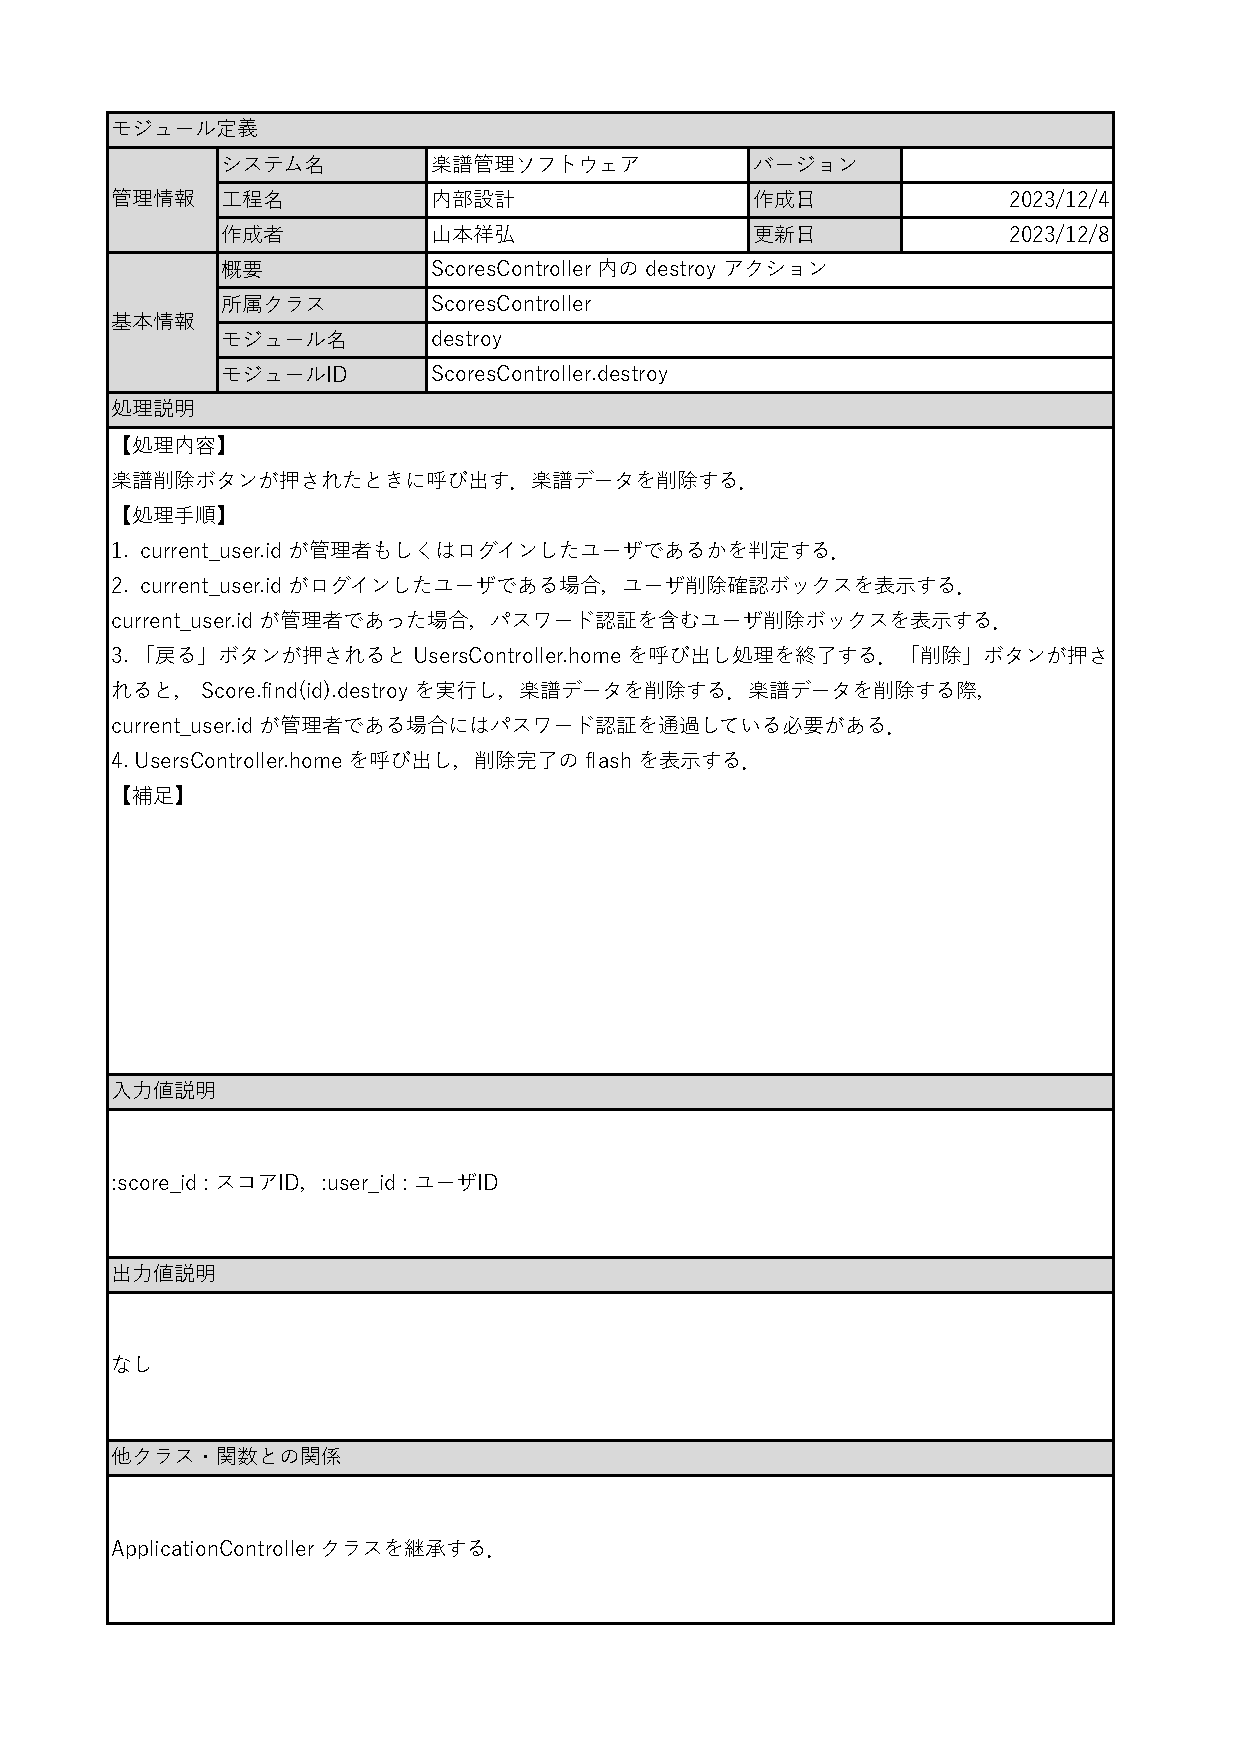
\includegraphics[scale=0.7]{img/Scores/xlsx/ScoresController_destroy.pdf}
    \vspace{-1cm}
    \caption{ScoresController.destroy定義書}
\end{figure}
\begin{figure}
    \centering
    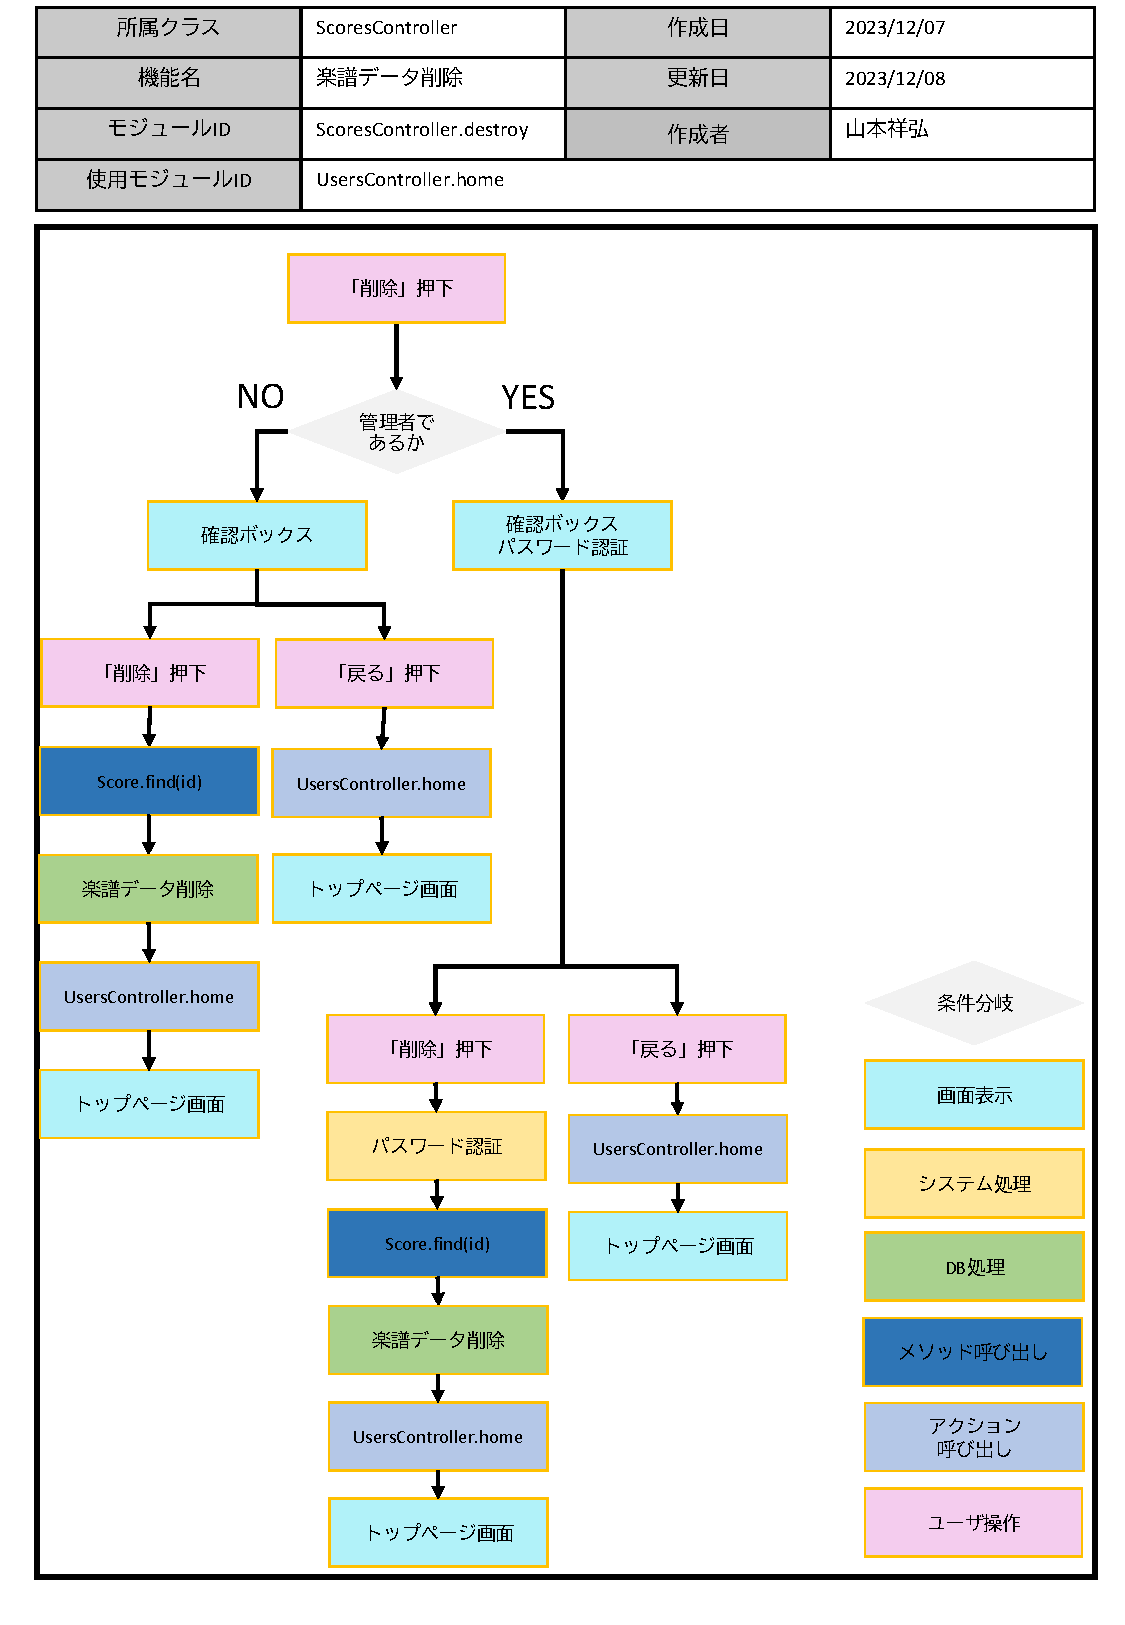
\includegraphics[scale=0.7]{img/Scores/pptx/ScoresController_destroy.pdf}
    \caption{ScoresController.destroyフロー図}
\end{figure}
\begin{figure}
    \centering
    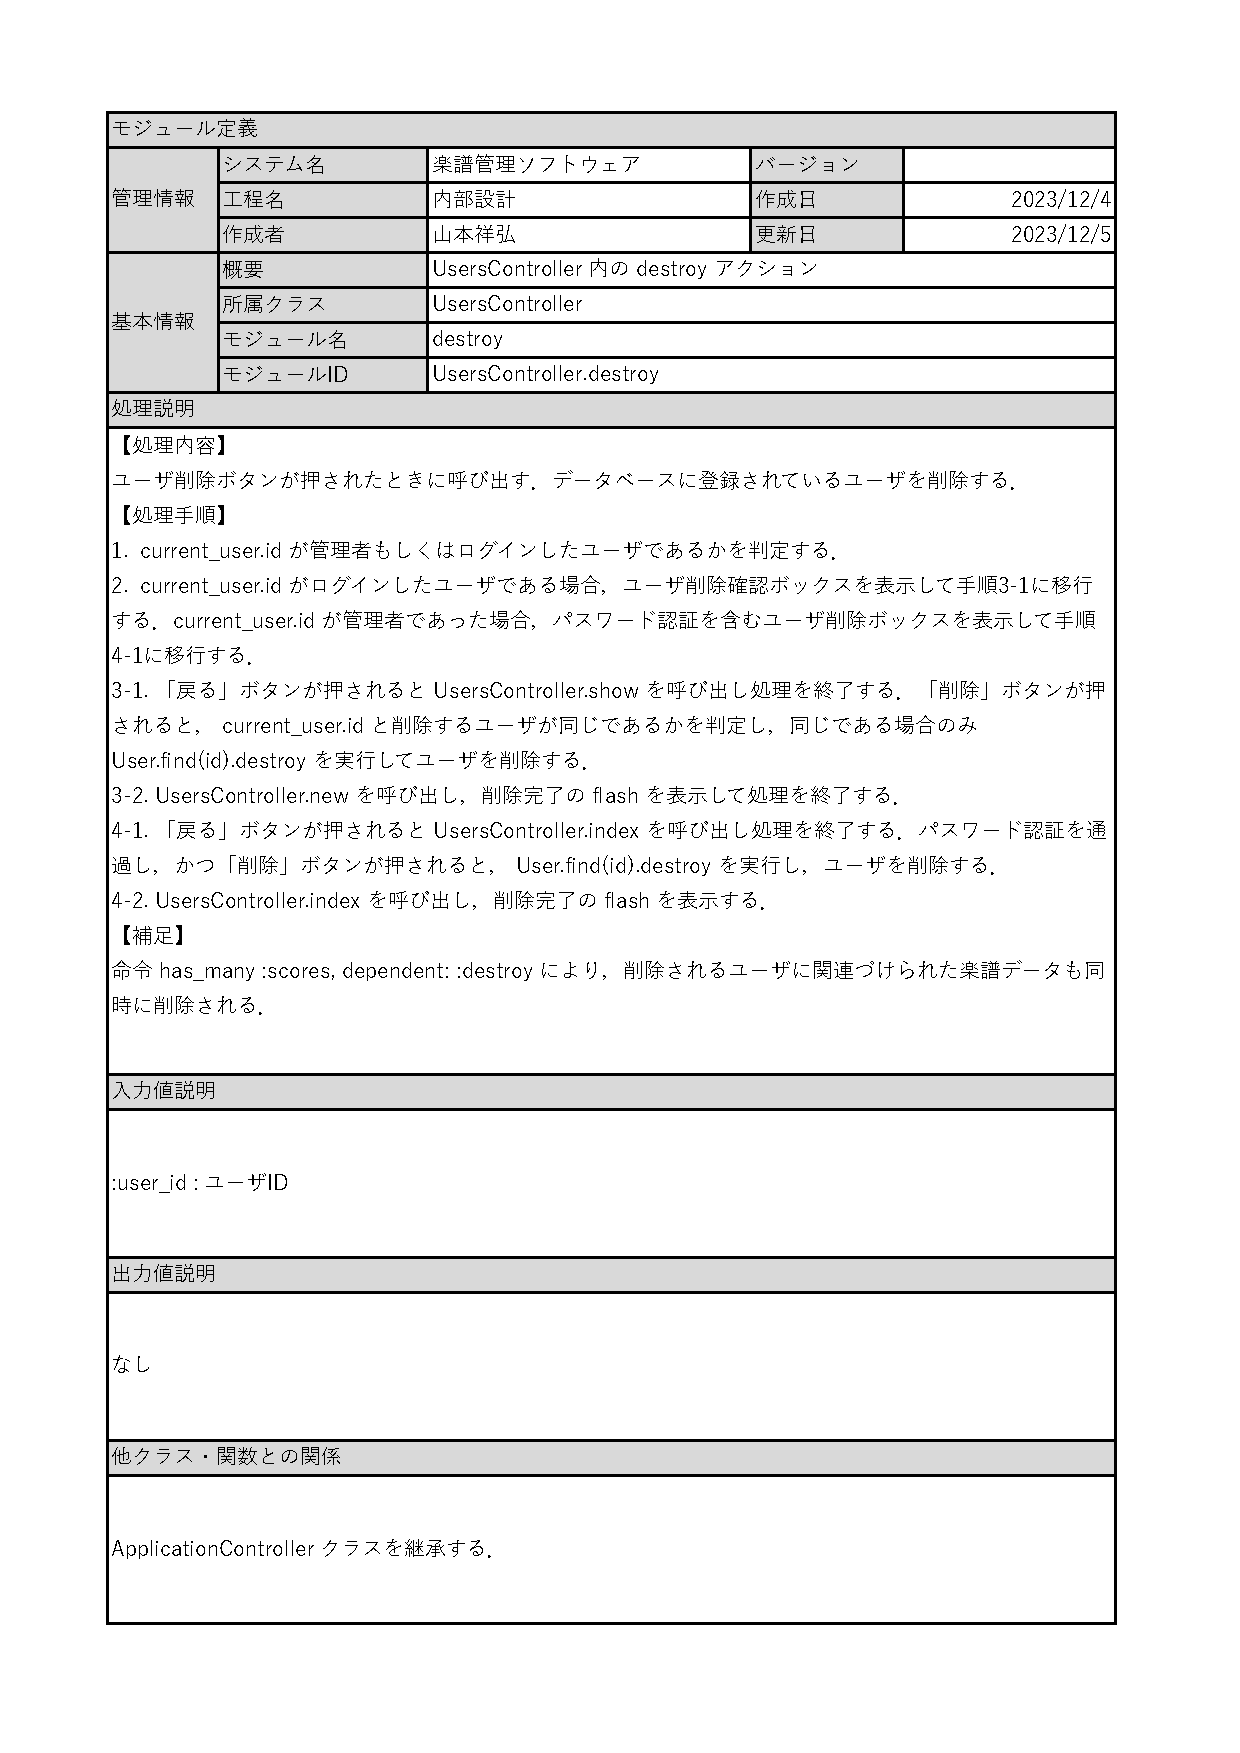
\includegraphics[scale=0.7]{img/Users/xlsx/UsersController_destroy.pdf}
    \vspace{-1cm}
    \caption{UsersController.destroy定義書}
\end{figure}
\begin{figure}
    \centering
    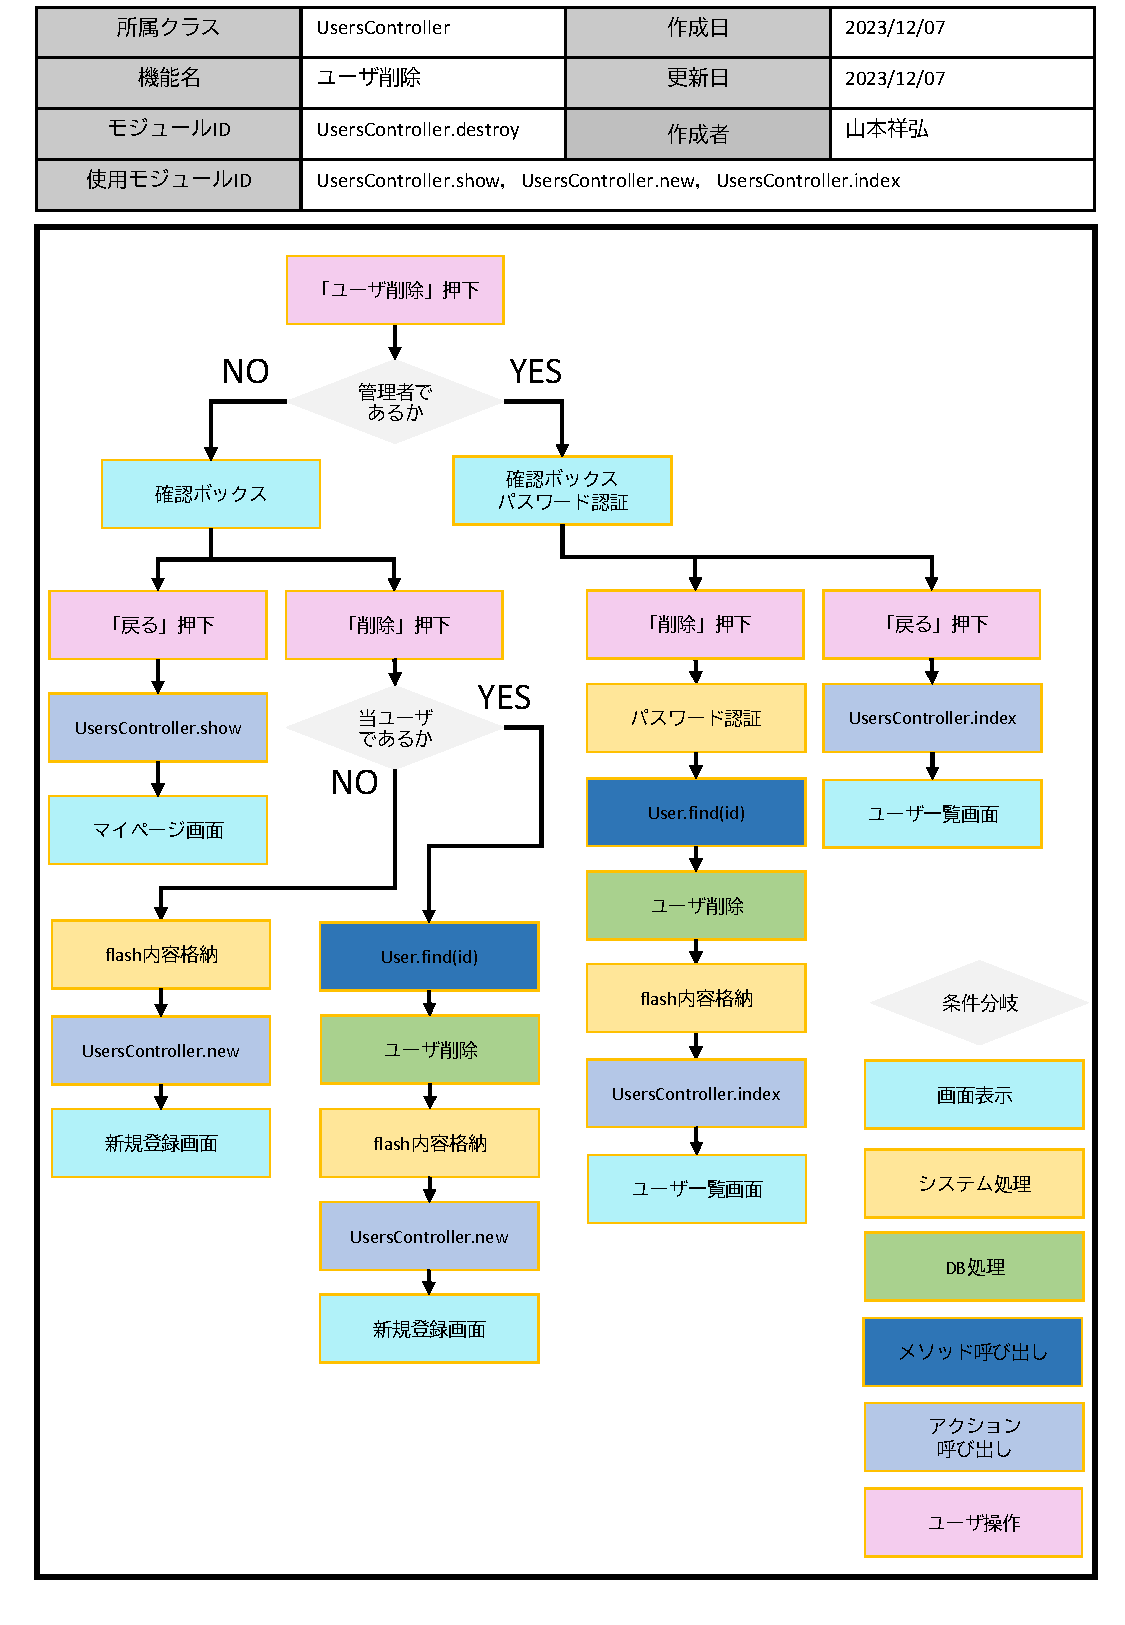
\includegraphics[scale=0.7]{img/Users/pptx/UsersController_destroy.pdf}
    \caption{UsersController.destroyフロー図}
\end{figure}


%session
\begin{figure}
    \centering
    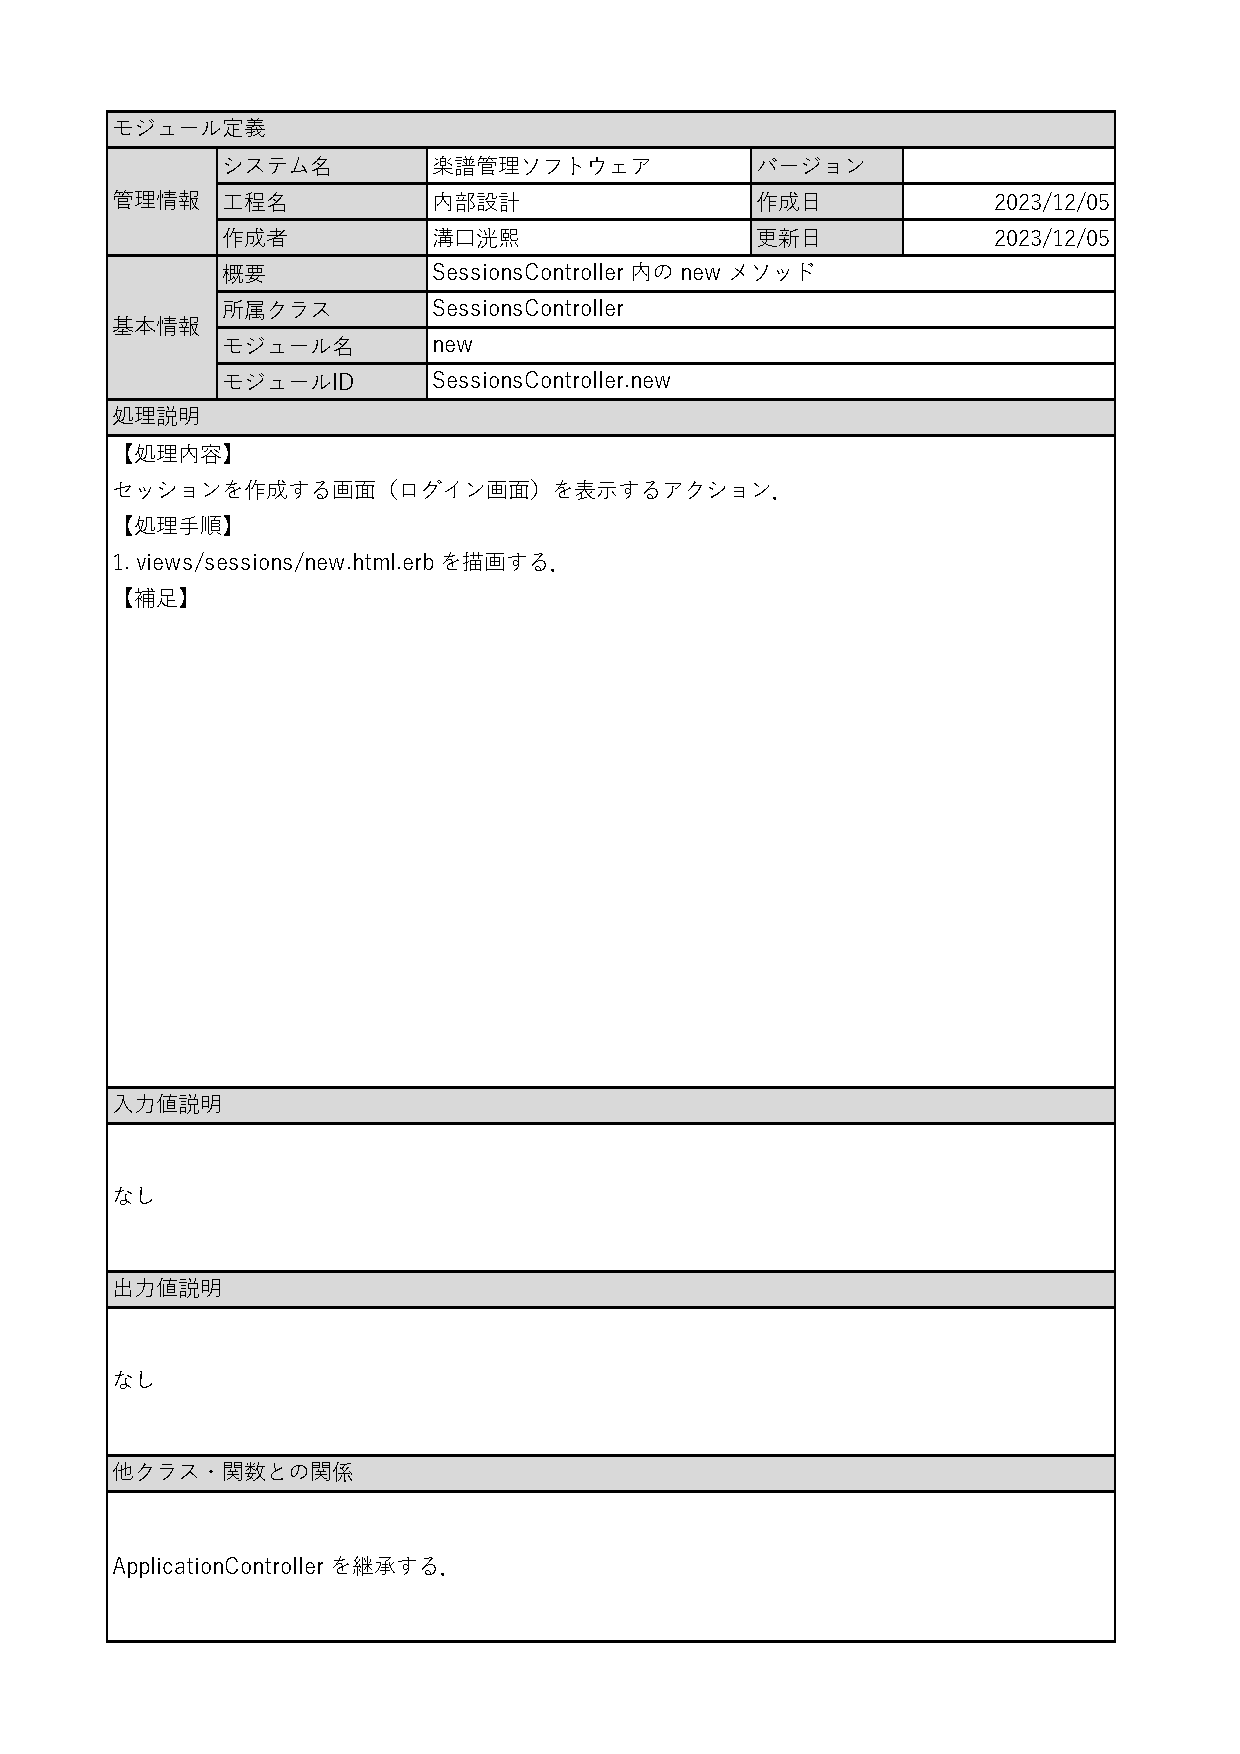
\includegraphics[scale=0.7]{img/Sessions/xlsx/SessionsController.new.pdf}
    \vspace{-1cm}
    \caption{SessionsController.new定義書}
\end{figure}
\begin{figure}
    \centering
    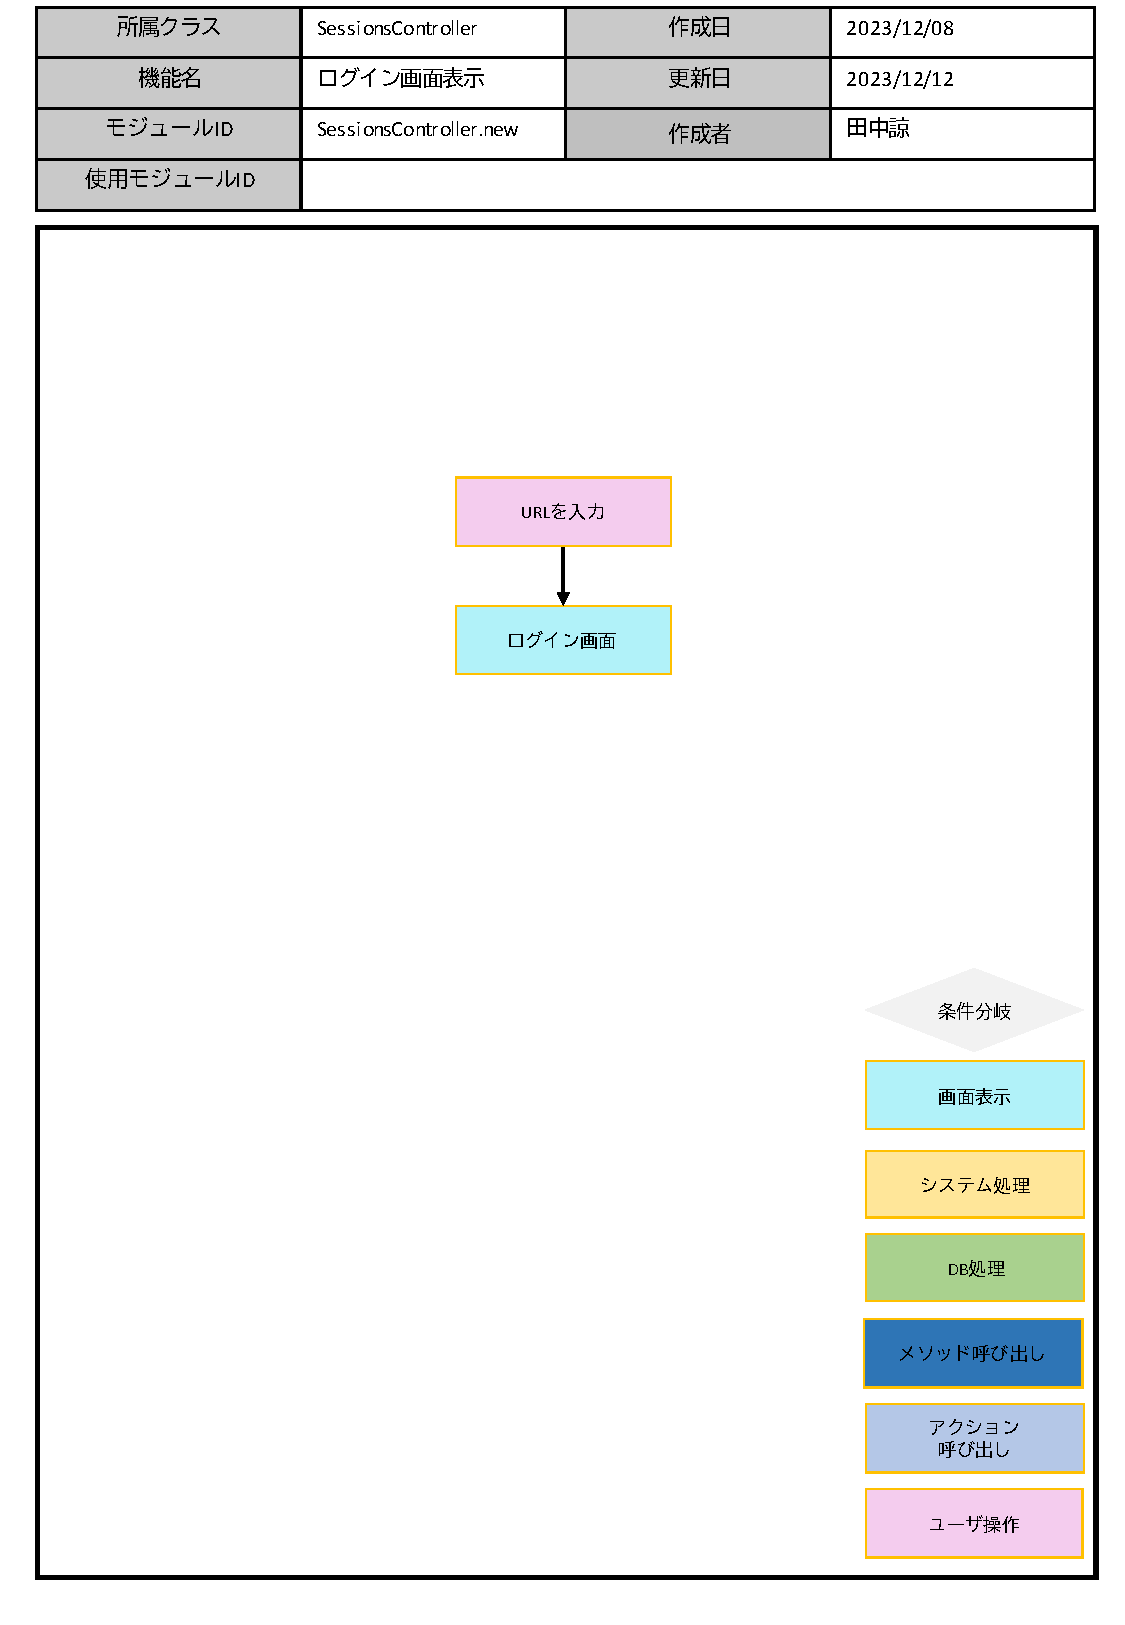
\includegraphics[scale=0.7]{img/Sessions/pptx/SessionsController_new.pdf}
    \caption{SessionsController.newフロー図}
\end{figure}
\begin{figure}
    \centering
    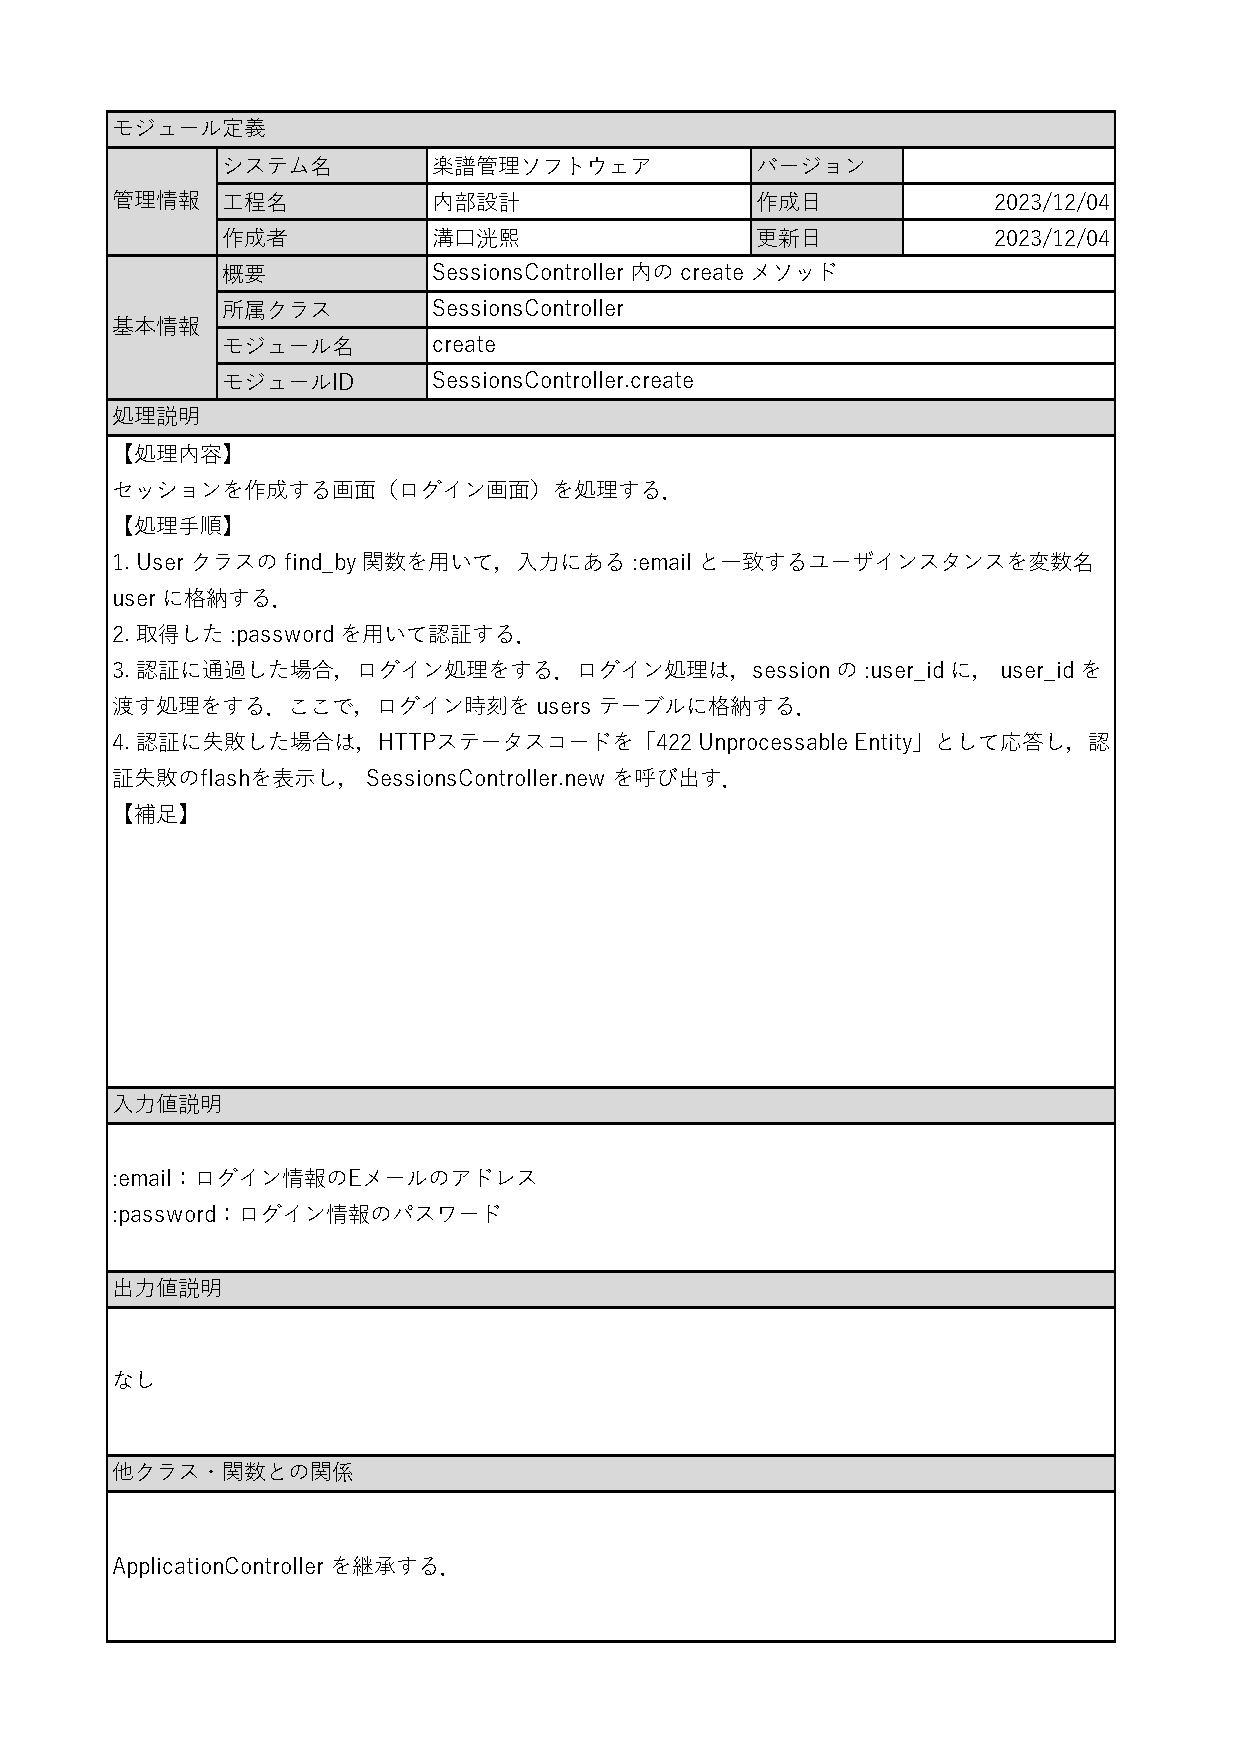
\includegraphics[scale=0.7]{img/Sessions/xlsx/SessionsController.create.pdf}
    \vspace{-1cm}
    \caption{SessionsController.create定義書}
\end{figure}
\begin{figure}
    \centering
    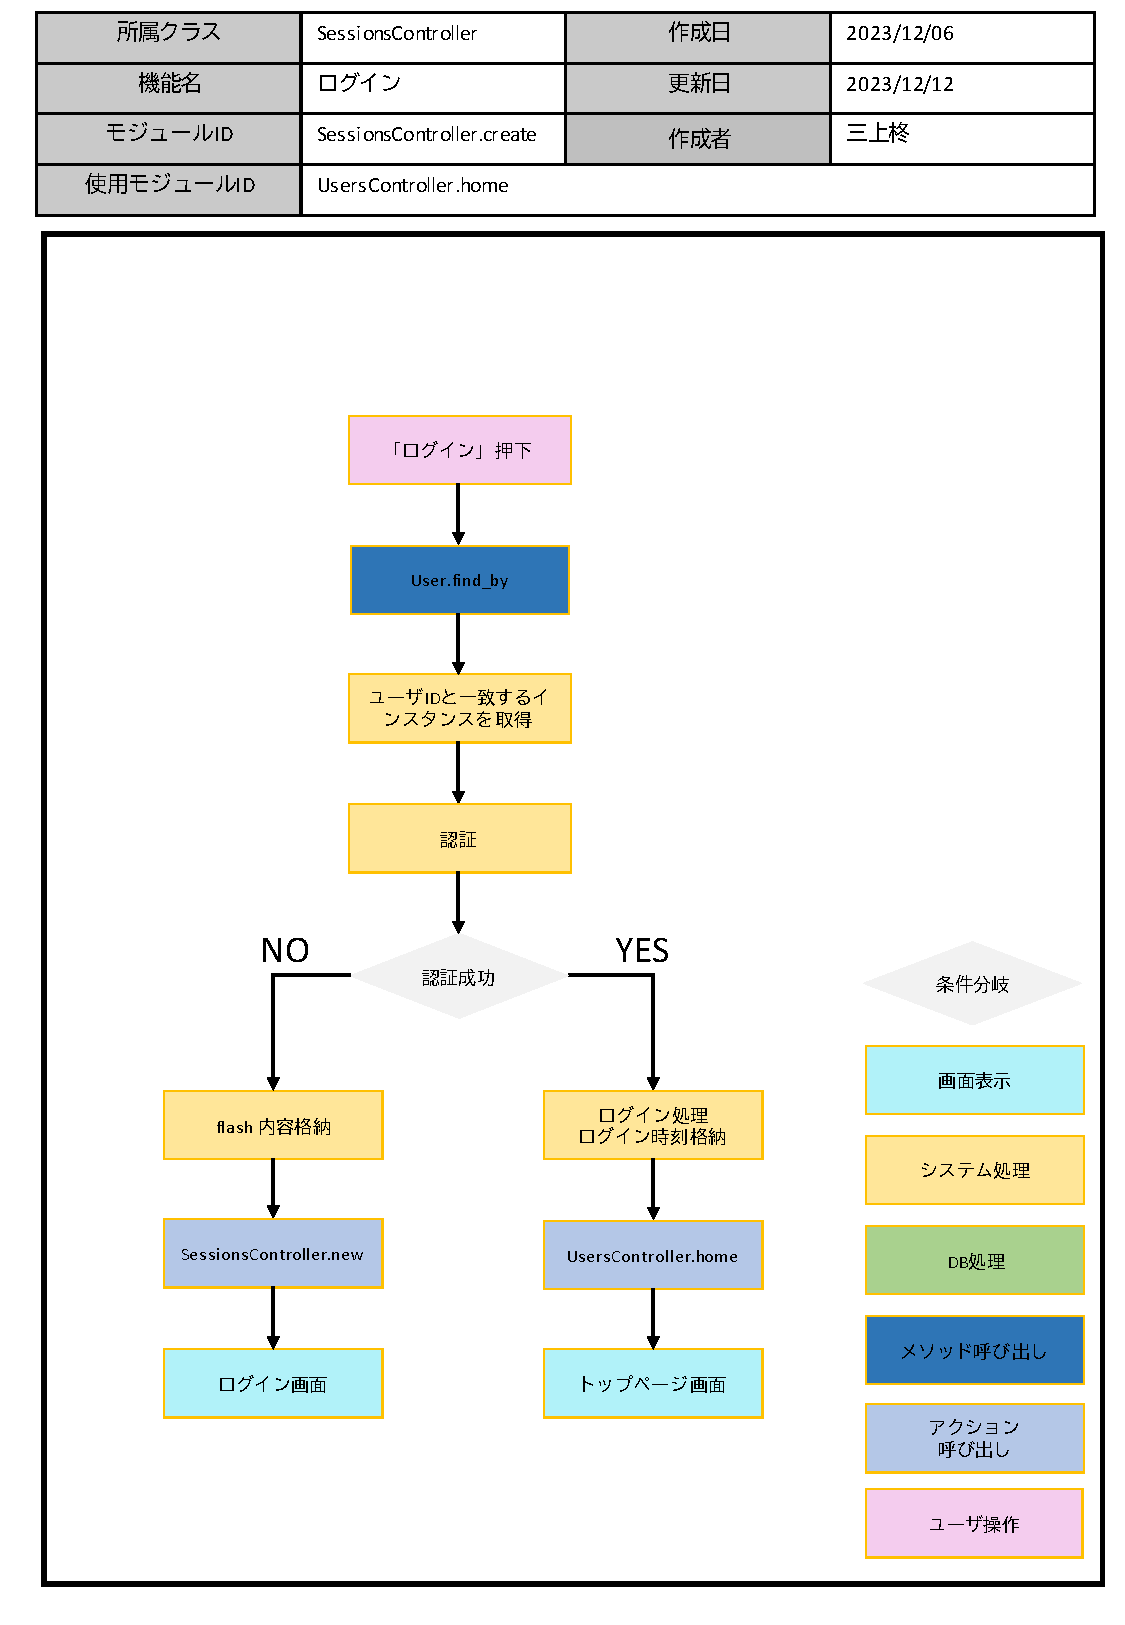
\includegraphics[scale=0.7]{img/Sessions/pptx/SessionsController_create.pdf}
    \caption{SessionsController.createフロー図}
\end{figure}
\begin{figure}
    \centering
    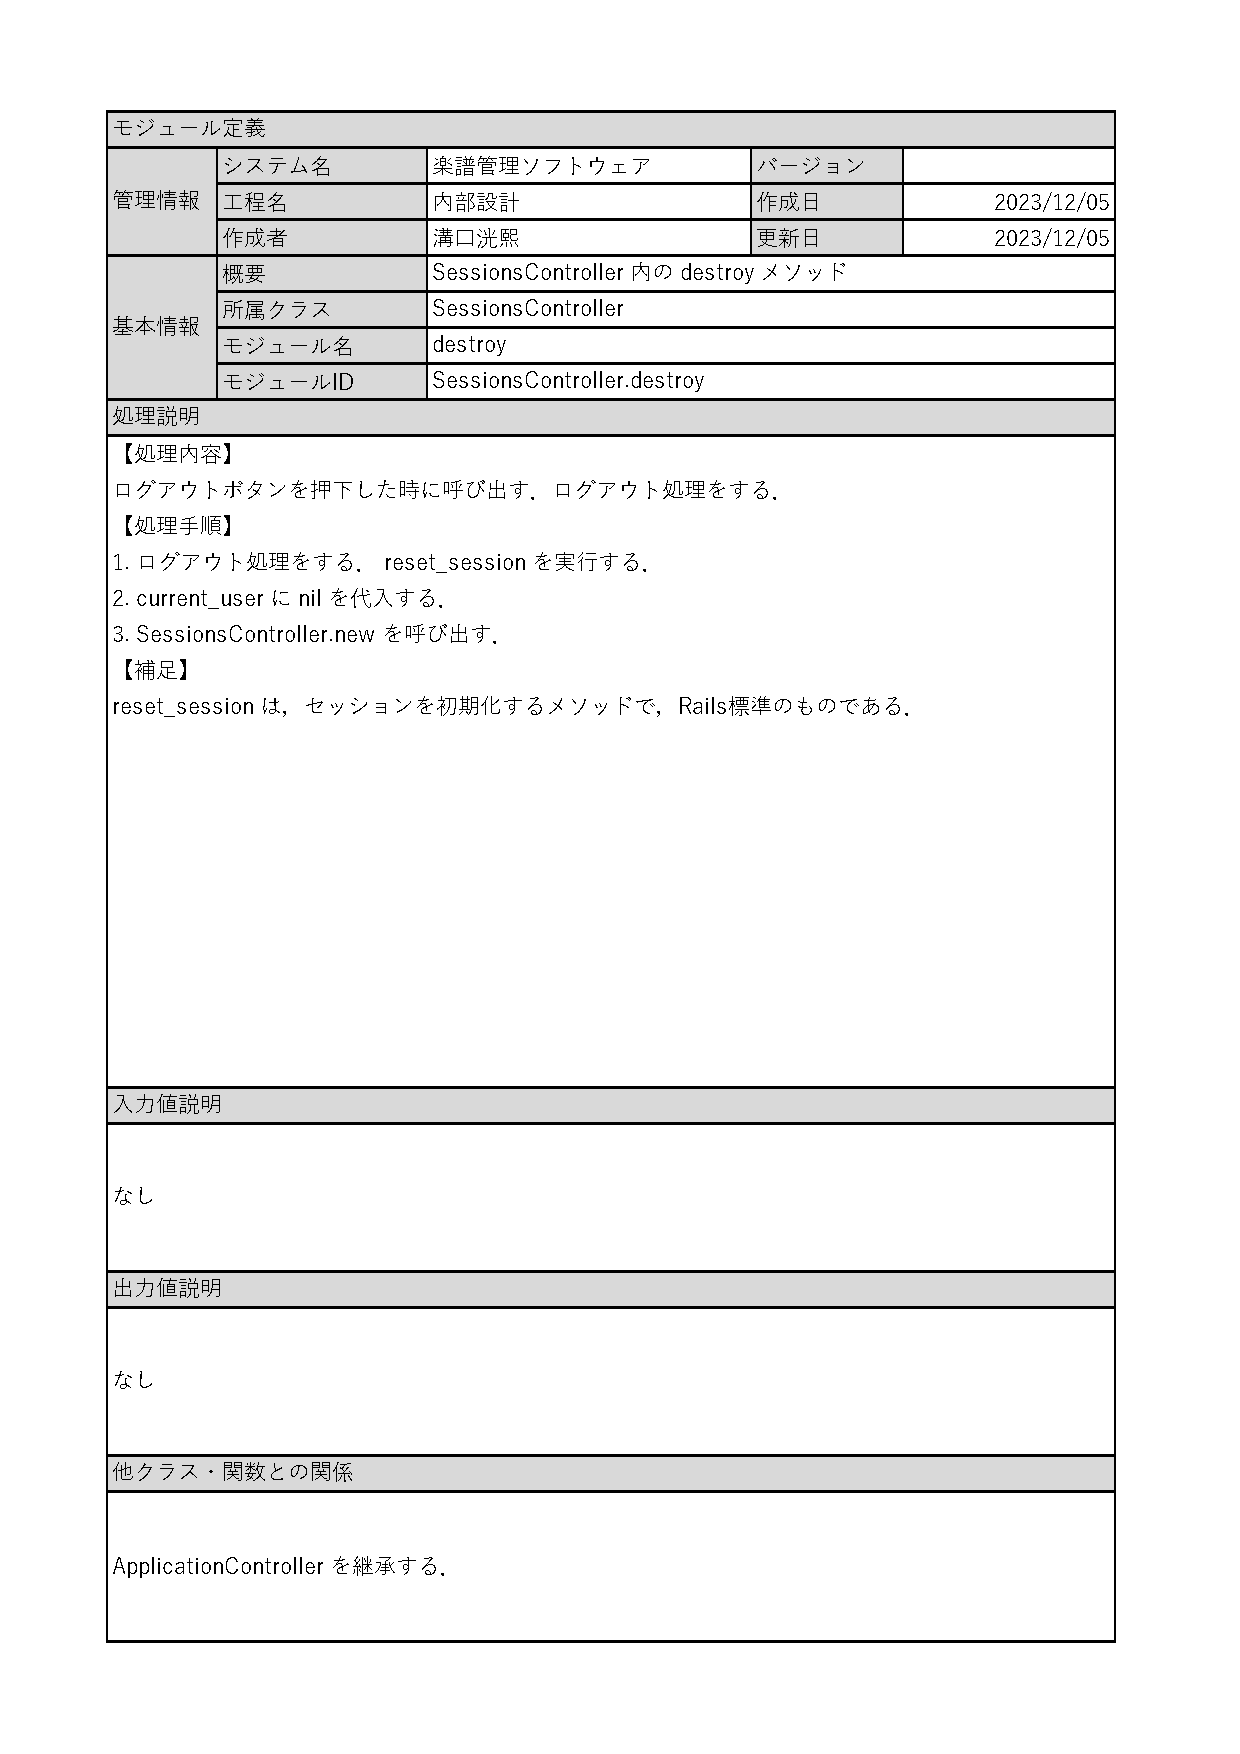
\includegraphics[scale=0.7]{img/Sessions/xlsx/SessionsController.destroy.pdf}
    \vspace{-1cm}
    \caption{SessionsController.destroy定義書}
\end{figure}
\begin{figure}
    \centering
    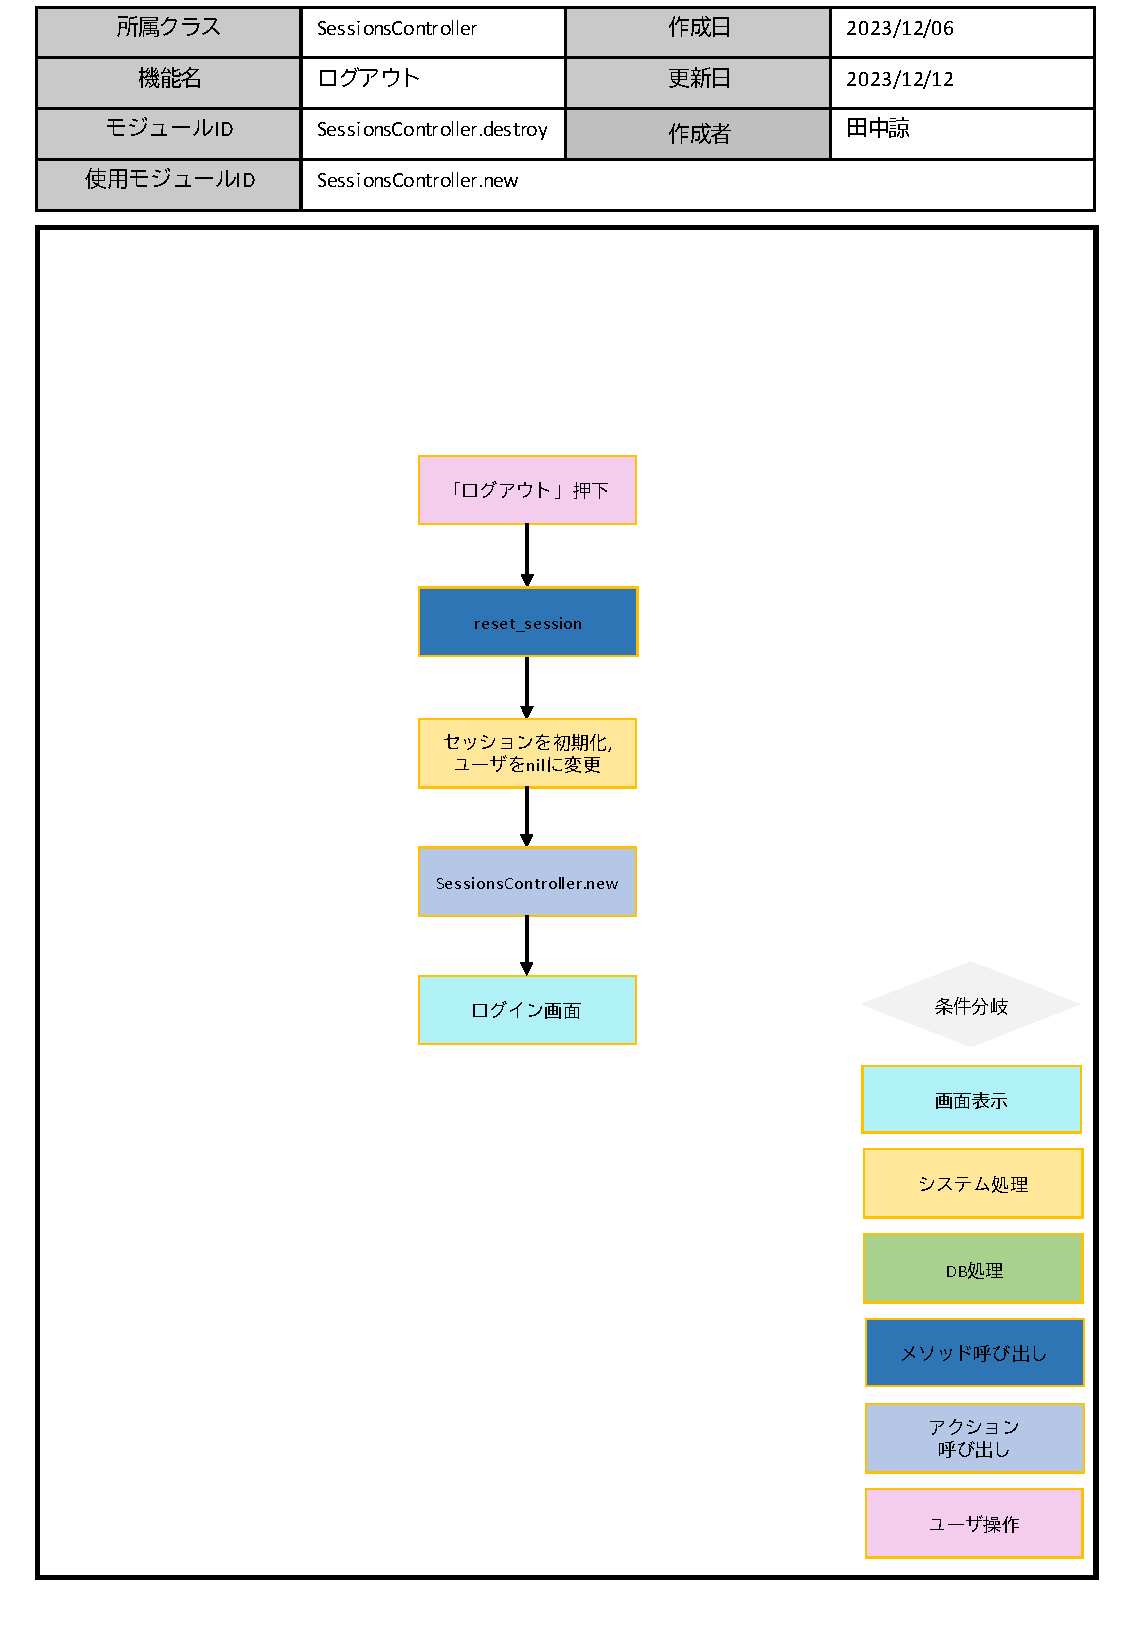
\includegraphics[scale=0.7]{img/Sessions/pptx/SessionsController_destroy.pdf}
    \caption{SessionsController.destroyフロー図}
\end{figure}
